%%%%%%%%%%%%%%%%%%%%%%%%%%%%%%%%%%%%%%%%%%%%%%%%%%%%%%%%%%%%%%%%%%%%%%%%%%%%%
%%
%% This file provides a template that can be used in concert with the
%% ohio-etd class to generate an electronic thesis or dissertation which
%% meets the formatting requirements at Ohio University.
%%
%% To use the template, copy this file (template.tex) and ohio-etd.cls into
%% the same directory and edit this template as required.  Reference
%% ohio-etd.pdf for additional instructions on using this class.
%%
%%%%%%%%%%%%%%%%%%%%%%%%%%%%%%%%%%%%%%%%%%%%%%%%%%%%%%%%%%%%%%%%%%%%%%%%%%%%%


%% Load the class.  Available options are: numbered, pdftex, cmfont,
%% singlespacetables, draft, 11pt, 12pt, leqno, and fleqn

\documentclass[numbered,pdftex]{ohio-etd}


%% Other packages that may be of use.  Delete or comment out (using a
%% percent sign in the first column) if they are not desired.  Reference
%% the corresponding documentation for more information on how to use these
%% packages.

\usepackage[square,sort&compress,numbers]{natbib} % Provides formatting for
                                                  % citations
\usepackage{textcomp} % Provides math symbols that can be used in text mode
\usepackage{amssymb}  % Provides additional AMS math symbols.  Note that
                      % amsmath is loaded as part of the ohio-etd class
\usepackage{bm}       % Provides bold-faced math symbols
\usepackage{booktabs} % Provides improved table formatting
\usepackage{dcolumn}  % Provides table columns aligned at decimal points
\usepackage{multirow} % Provides table elements spanning multiple rows
\usepackage{graphicx} % Standard package to incorporate graphics
\usepackage[printonlyused]{acronym} % Provides a method for incorporating
                                    % acronyms and building an acronym list
                                    
\usepackage[T1]{fontenc}
\usepackage{ragged2e}

\graphicspath{{figures/}} % Allows graphics files to be stored in a
                          % separate directory



%% Required front matter definitions

\degree    {MS}              % MS, MA, MCTP, or PhD
\graduation{May}{2021}    % May, August, or December 

\title     {LSTMs and Deep Residual Networks for Carbohydrate and Bolus Recommendations in Type 1 Diabetes Management}
\author    {Jeremy T.}{Beauchamp} 

\advisor   {Razvan Bunescu}{Associate Professor}
\dean      {Mei Wei}{Dean and Moss Professor of Engineering Education}

\program   {Computer Science}            % e.g. Electrical Engineering
\department{School of Electrical Engineering and Computer Science} % e.g. School of Electrical Engineering 
                                     %      and Computer Science
\college   {Russ College of Engineering and Technology}   % e.g. Russ College of Engineering and
                                     %      Technology

\abstract{
\justifying
To avoid serious diabetic complications, people with type 1 diabetes must keep their \ac{BGLs} as close to normal as possible. Insulin dosages and carbohydrate consumption are important considerations in managing \ac{BGLs}. Since the 1960s, models have been developed to forecast blood glucose levels based on the history of \ac{BGLs}, insulin dosages, carbohydrate intake, and other physiological and lifestyle factors. Such predictions can be used to alert people of impending unsafe \ac{BGLs} or to control insulin flow in an artificial pancreas. In past research, an LSTM-based approach to blood glucose level prediction was developed to process "what if" scenarios, in which people could enter foods they might eat or insulin amounts they might take and then see the affect on future \ac{BGLs}. In this work, the "what-if" scenario is inverted and a similar architecture is introduced, based on chaining two LSTMs that can be trained to make either insulin or carbohydrate recommendations aimed at reaching a desired BG level in the future. Leveraging a recent state-of-the-art model for time series forecasting, a novel deep residual architecture is proposed for the same recommendation task, in which the two LSTM chain is used as a repeating block. Experimental evaluations using real patient data from the OhioT1DM dataset show that the new integrated architecture compares favorably with the previous LSTM-based approach, substantially outperforming the baselines. The promising results suggest that this novel approach could potentially be of practical use to people with type 1 diabetes for self-management of \ac{BGLs}.}

%To avoid serious diabetic complications, people with type 1 diabetes must keep their blood glucose levels (BGLs) as close to normal as possible. Insulin dosages and carbohydrate consumption are important considerations in managing BGLs. Since the 1960s, models have been developed to forecast blood glucose levels based on the history of BGLs, insulin dosages, carbohydrate intake, and other physiological and lifestyle factors. Such predictions can be used to alert people of impending unsafe BGLs or to control insulin flow in an artificial pancreas. In past work, we have introduced an LSTM-based approach to blood glucose level prediction aimed at "what if" scenarios, in which people could enter foods they might eat or insulin amounts they might take and then see the effect on future BGLs. In this work, we invert the "what-if" scenario and introduce a similar architecture based on chaining two LSTMs that can be trained to make either insulin or carbohydrate recommendations aimed at reaching a desired BG level in the future. Leveraging a recent state-of-the-art model for time series forecasting, we then derive a novel architecture for the same recommendation task, in which the two LSTM chain is used as a repeating block inside a deep residual architecture. Experimental evaluations using real patient data from the OhioT1DM dataset show that the new integrated architecture compares favorably with the previous LSTM-based approach, substantially outperforming the baselines. The promising results suggest that this novel approach could potentially be of practical use to people with type 1 diabetes for self-management of BGLs.

%% Optional front matter definitions.  Delete or comment out if not needed

%\coadvisor {Coadvisor's Full Name}{Coadvisor's Full Title}

%\dedication{}

\acknowledgments{
I would like to thank my advisor Dr. Razvan Bunescu for his exceptional guidance, knowledge, and mostly, his patience and professionalism. I have had the pleasure of learning a lot from Dr. Bunescu and this research certainly would not have been possible without him. I would also like to thank Dr. Cindy Marling for all of her assistance and knowledge throughout the research process. In addition, I would like to thank Zhongen Li for his help implementing parts of this project.
}

%% If you prefer to provide "acknowledgements" instead (note the added "e"
%% between the "g" and the "m") then add the "e" in the macro name so that
%% it reads "\acknowledgements".}

%% Additional "lists" can be added to the end of the front matter using the
%% \addlistof macro.  For example:
%\addlistof{Symbols}{Insert your list of symbols here or comment out this line.}
%% Note that the command "\input{symbols}" can be used if the symbol list is
%% contained in a separate file called "symbols.tex"}

%\addlistof{Acronyms}{
\addlistof{Acronyms}{
	\begin{acronym}
	    \acro{BG}{Blood Glucose}
	    \acro{BGL}{Blood Glucose Level}
	    \acro{BGLs}{Blood Glucose Levels}
	    \acro{BGLP}{Blood Glucose Level Prediction}
	    \acro{BW}{Bolus Wizard}
	    \acro{CGM}{Continuous Glucose Monitor}
	    \acro{FC}{Fully Connected}
	    \acro{FCN}{Fully Connected Network}
	    \acro{LSTM}{Long-Short Term Memory}
	    \acro{MAE}{Mean Absolute Error}
	    \acro{N-BEATS}{Neural Basis Expansion for Interpretable Time-Series Forecasting}
	    \acro{RMSE}{Root Mean Square Error}
	    \acro{RNN}{Recurrent Neural Network}
	    \acro{RNNs}{Recurrent Neural Networks}
		\acro{T1D}{Type 1 Diabetes}
		\acro{T2D}{Type 2 Diabetes}
		\acro{ToD}{Time-of-Day}
	\end{acronym}
}
%}

%% Use "\addlistof{Acronyms}{
	\begin{acronym}
	    \acro{BG}{Blood Glucose}
	    \acro{BGL}{Blood Glucose Level}
	    \acro{BGLs}{Blood Glucose Levels}
	    \acro{BGLP}{Blood Glucose Level Prediction}
	    \acro{BW}{Bolus Wizard}
	    \acro{CGM}{Continuous Glucose Monitor}
	    \acro{FC}{Fully Connected}
	    \acro{FCN}{Fully Connected Network}
	    \acro{LSTM}{Long-Short Term Memory}
	    \acro{MAE}{Mean Absolute Error}
	    \acro{N-BEATS}{Neural Basis Expansion for Interpretable Time-Series Forecasting}
	    \acro{RMSE}{Root Mean Square Error}
	    \acro{RNN}{Recurrent Neural Network}
	    \acro{RNNs}{Recurrent Neural Networks}
		\acro{T1D}{Type 1 Diabetes}
		\acro{T2D}{Type 2 Diabetes}
		\acro{ToD}{Time-of-Day}
	\end{acronym}
}" if the acronym list is in a separate file called
%% "acronyms.tex".  Note that the formatting generated by the acronym package
%% can be forced into singlespaced text by inserting "\setlength\itemsep{0pt}
%% \setlength\parskip{0pt}" into the "acronym" environment.} 

%% For documents created by government employees as part of their
%% employment.  The wording of the disclaimer can be specified using an
%% option.  See the documentation for more information.

% \govtdisclaimer    

% \notables  % Prevent a list of tables from being created
% \nofigures % Prevent a list of figures from being created

\begin{document}
\justifying

\makefrontmatter    % Creates all of the front matter pages.

%% Body of the text follows, using \chapter, \section, \subsection,
%% \subsubsection, \paragraph, and \subparagraph to generate the
%% section headings.  For convenience, it may be useful to break the
%% full document into separate files, perhaps divided by chapters.  In
%% that case, the files would be loaded here using "\input{filename}"

\chapter{Introduction}
\label{chapter:introduction}

Diabetes is a disease in which the body either does not produce enough insulin or cannot make sufficient use of the insulin that it does produce. Insulin is a critical hormone that allows the glucose from the blood stream to be absorbed into cells. Without it, or a way for the body to properly process it, too much glucose remains in the bloodstream. High amounts of glucose in the bloodstream can lead to several serious complications, including heart disease, vision loss, and kidney disease \cite{CDC:diabetes}. There are two major types of diabetes, \ac{T1D} and \ac{T2D}, both of which require careful management of \ac{BGLs}. %blood glucose levels (BGLs).

In \ac{T1D}, which is the most severe type of diabetes, the pancreas does not produce insulin, which leads to BG levels that are too high \cite{CDC:diabetes}. This is thought to be caused by the destruction of cells in the pancreas by an autoimmune reaction. Of all people diagnosed with diabetes, only about 5-10\% of them have type 1 \cite{CDC:diabetes}. Those with \ac{T1D} typically are diagnosed with it early in life. As of now, there is no known cure or prevention measure for \ac{T1D}.

In \ac{T2D}, the body does not use insulin efficiently enough to keep \ac{BGLs} at normal levels. Type 2 accounts for about 90-95\% of all cases of diabetes \cite{CDC:diabetes}. Fortunately, \ac{T2D} can be prevented or delayed by living a generally healthy lifestyle.

The day-to-day self-management of diabetes is essential for someone with \ac{T1D}. The patient must painstakingly manage their \ac{BGLs} and attempt to prevent them from becoming too high or too low. \ac{T1D} is managed by using external sources of insulin to prevent \ac{BGLs} from becoming too high. However, much care must be put into the amount of insulin that is allowed into the body. Too much insulin can cause \ac{BGLs} to drop too low. When \ac{BGLs} become too high, patients may begin to experience symptoms of hyperglycemia. When \ac{BGLs} drop too low, patients will likely start to feel the effects of hypoglycemia. Both hyperglycemia and hypoglycemia are dangerous and can lead to severe long-term complications if \ac{BGLs} are not promptly corrected.

An important part of diabetes management consists of vigilantly monitoring one's \ac{BGL}. One way this can be done is by using a glucometer, which measures the amount of glucose in a blood sample, typically taken from a fingertip. Another common method of monitoring \ac{BGLs} is by using a \ac{CGM} system, a device capable of measuring blood glucose every few minutes via a subcutaneous sensor \cite{CDC:managing}. A person with \ac{T1D} must also make key decisions about how much insulin to take and when to take it several times per day. They must also make decisions about the quantity and timing of their meals throughout the day.

Diabetes management primarily involves taking actions to correct \ac{BGL} issues as they arise. Once \ac{BGLs} become too high a person will \emph{react} to this by taking insulin. Likewise, a person will \emph{react} to their \ac{BGLs} dropping too low by eating or taking glucose tablets. The process of diabetes management could potentially be simpler and even safer if a more proactive approach was taken instead. Rather than reacting to symptoms of hyperglycemia or hypoglycemia, preemptive steps could be taken to prevent these symptoms altogether.

An important step towards more proactive diabetes management is the ability to forecast future \ac{BGLs} accurately. This information would allow people to make more informed decisions about how to prevent potential hypoglycemic or hyperglycemic events. Efforts to model \ac{BGLs} can be dated back to as early as the 1960s \cite{boutayeb2016}. In recent years, there has been much research into using machine learning algorithms for blood glucose level prediction \cite{plis:maiha14, rubin_falcone:nbeats_bgl, mirshekarian:bgl_pred, bunescu:svr_bgl}. With the widespread adoption of \ac{CGM} systems, and the large amounts of data that they can collect, machine learning has become a more feasible approach to create \ac{BGL} prediction systems. However, even with the ability to forecast \ac{BGLs}, the patient would still need to make a decision about how much to eat to raise their \ac{BGLs} to a normal range or how much to bolus to lower their \ac{BGLs} to a healthy level. This kind of decisions are the primary focus of this thesis.

%However, even with the ability to forecast BGLs, the patient would still need to make a decision about how much to eat/bolus to raise/lower their BGLs to a healthier range or to maintain their current blood glucose level. This is the primary focus of this thesis.

\section{Research Objective}
\label{section:objective}
The objective of the research presented in this thesis is to design and train neural network models capable of providing people with \ac{T1D} recommendations on how many grams of carbohydrates they should eat or how much insulin they should bolus to reach a target \ac{BGL} in the near future. This can be thought of as essentially reversing the \ac{BGL} prediction problem. Instead of predicting \ac{BGLs} in the near future, the objective of this research is to recommend an action that a person should take in order to reach a desired \ac{BGL} in the near future. Previous research in \ac{BGL} prediction \cite{mirshekarian:bgl_pred} has aimed to answer the question of "What will my \ac{BGL} be in an hour if I eat a 30 carbs snack 10 minutes from now?", while this research attempts to answer the question "How many carbs should I eat 10 minutes from now to raise my \ac{BGL} to 140 in an hour?". Two architectures are developed for these tasks, an LSTM-based architecture and an N-BEATS-based architecture. The LSTM-based architecture draws inspiration from the architecture introduced in \cite{mirshekarian:bgl_pred} for the task of \ac{BGL} prediction. The architecture was redesigned to make meal or bolus recommendations using similar input data to that of the original \ac{BGL} prediction system. The N-BEATS-based architecture is a modified version of the original N-BEATS architecture \cite{oreshkin:nbeats}, taking inspiration from another modified version of the N-BEATS architecture that was built for the task of \ac{BGL} prediction \cite{rubin_falcone:nbeats_bgl}. Both architectures are trained on the OhioT1DM dataset \cite{ohiot1dm:marling:kdh18}, which contains data from real people with \ac{T1D}. The goal of this research is to use this real-patient data and proven \ac{BGL} prediction architectures to create accurate, personalized bolus and meal recommendation systems.

%The contribution of this thesis is a general neural network architecture that can be trained to make bolus recommendations and meal recommendations. Two architectures were developed and compared on the tasks of bolus and carbohydrate recommendations, an LSTM-based architecture and an N-BEATS-based architecture. The LSTM-based architecture draws inspiration from the architecture introduced in \cite{mirshekarian:bgl_pred} for the task of BGL prediction. The architecture was redesigned to make meal or bolus recommendations using similar input data to that of the original BGL prediction system. The N-BEATS-based architecture is based on the original N-BEATS architecture \cite{oreshkin:nbeats}, and the modified version that was built for the task of BGL prediction \cite{rubin_falcone:nbeats_bgl}. Our N-BEATS-based architecture makes additions to these architectures which make them better suited for the tasks of bolus and meal recommendations. Both architectures are trained on the OhioT1DM dataset \cite{ohiot1dm:marling:kdh18}, which contains data from real people with T1D. The goal of this research is to use real-patient data and proven BGL prediction architectures to create accurate, personalized bolus and meal recommendation systems.

\section{Thesis Outline}
\label{section:structure}
The rest of this thesis is structured as follows:

\begin{itemize}
	\item Chapter \ref{chapter:background} will compare and contrast this research with other similar research, as well as provide background on some of the core deep learning models that are utilized in this work.
	\item Chapter \ref{chapter:models} will characterize the problems that this research aims to solve as well as the neural architectures that have been designed for each recommendation scenario.
	\item Chapter \ref{chapter:data} will introduce the dataset that is used for this research as well as the pre-processing procedures that have been developed for mitigating the noise in the original raw data.
	\item Chapter \ref{chapter:methods} will explain the procedures for training and evaluating the models, as well as discuss the results of several experimental evaluations.
	\item Chapter \ref{chapter:conclusion} will end this thesis with concluding remarks and suggestions for future research.
\end{itemize}


\chapter{Background}
\label{chapter:background}

This chapter will provide background on the major neural network architectures that are utilized in this research, as well as summarize and discuss research related to artificial intelligence-based \ac{T1D} management systems. Two of the most common \ac{T1D} management systems are \ac{BGL} prediction systems and insulin recommendation systems. Research into improving the accuracy and reliability of these systems could have a significant positive impact on the lives of those with \ac{T1D}. These systems can give people with \ac{T1D} more confidence in their decisions about how much insulin they should take and provide insight into how these decisions will affect their \ac{BGLs} over the following hours. As artificial intelligence and machine learning algorithms continue to evolve and improve, so too can the performance of these \ac{T1D} management systems.

\section{Time Series Prediction Models}
\label{section:time_series}

Neural networks are powerful machine learning models capable of learning to perform a wide variety of tasks across many domains given sufficient training data. In this research, the goal is to create neural network models capable of performing time series forecasting, where the task consists of predicting a future point in a time series given previous data from the series. However, due to the temporal nature of the data, a generic fully connected neural network will have difficulty processing time series data. As described in the following sections, \ac{RNNs} and Deep Residual Networks are two types of networks that are capable of processing and learning from such data.

\subsection{Recurrent Neural Networks}
\label{section:rnn}

\begin{figure*}[t]
    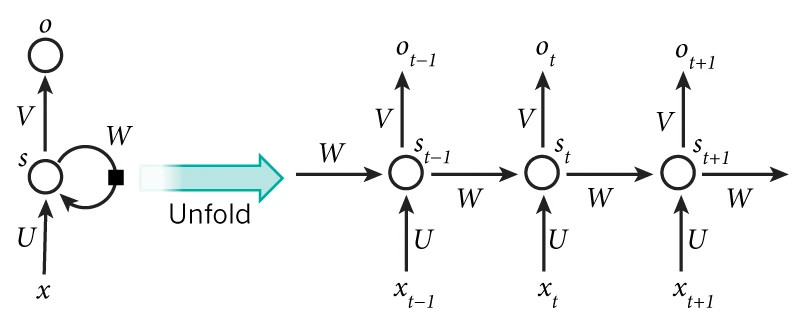
\includegraphics[width=\textwidth]{rnn}
    \caption{A visualization of an RNN \cite{lecun2015deep}.}
    \label{fig:rnn}
\end{figure*}

\ac{RNNs} are neural networks capable of learning from time series data. \ac{RNNs} process time series data in discrete time-steps, rather than processing all of it at once like a fully connected network would. \ac{RNNs} have three sets of weights, $W$, $U$, and $V$, that are used to compute a hidden state, $\text{{\bf s}}_{t}$ and an output $\text{{\bf o}}_t$ for every time step $t$. The state contains values that the network has recursively computed based on inputs from all previous time-steps. Along with the hidden state of the previous time-step, $\text{{\bf s}}_{t-1}$, the input at the current step in the time series, $\text{{\bf x}}_t$, is used to calculate both the output of the cell and the hidden state values. The hidden state at time $t$, $\text{{\bf s}}_t$, is calculated by the following formula:

\begin{center}
   $\text{{\bf s}}_t = f(W\text{{\bf s}}_{t-1} + U\text{{\bf x}}_{t} + \text{{\bf b}}_s)$
\end{center}
where $\text{{\bf b}}_s$ is a bias vector, and $f$ is a non-linear activation function. The tanh function or the sigmoid function are common choices for $f$. The output of the network at time $t$, $\text{{\bf o}}_t$, is calculated as follows:

\begin{center}
    $\text{{\bf o}}_t = f(V\text{{\bf s}}_{t} + \text{{\bf b}}_o)$
\end{center}
where $f$ is again a non-linear activation function and $\text{{\bf b}}_o$ is a different bias vector. Note that $f$ does not need to be the same in both equations. The weight matrices $W$, $U$, $V$, are learned via the Backpropagation Through Time (BPTT) algorithm \cite{werbos:bptt}. While \ac{RNNs} are capable of learning from time series data, they can have difficulty learning long distance dependencies due to the vanishing gradient problem \cite{bengio:vanishing}. The vanishing gradient problem refers to norm of the gradient rapidly shrinking to 0 for long-term dependencies during training, which makes it very difficult for \ac{RNNs} to learn the relationships between events that are temporally distant \cite{pascanu2013difficulty}. While there have been several proposed \ac{RNN} modifications that aim to remedy this issue, one of the most widely used is the \ac{LSTM} network \cite{hochreiter:nc97}.

\subsubsection{Long Short-Term Memory}
\label{section:lstm_background}

\begin{figure*}[t]
    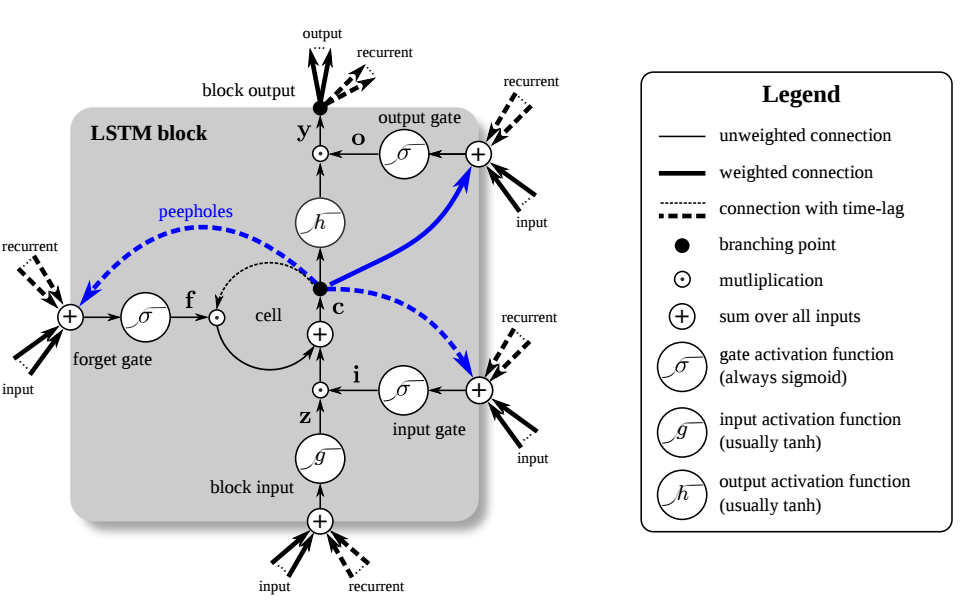
\includegraphics[width=\textwidth]{lstm}
    \caption{A diagram of an LSTM cell. The peephole connections represented by the blue lines are not part of the original LSTM architecture. Image from \cite{greff2016lstm} was slightly modified.}
    \label{fig:lstm}
\end{figure*}

In 1997, \ac{LSTM} networks were introduced as a solution to the vanishing gradient problem \cite{hochreiter:nc97}. \ac{LSTM} networks use multiplicative gates on the input and output for each cell. The purpose of the input gate is to prevent the information that has already been learned from the sequence to be perturbed by input events that are not relevant. Similarly, the output gate prevents irrelevant information from negatively affecting the output of a particular cell. In addition to gating the inputs and outputs of a cell, \ac{LSTM} cells also include a forget gate, which allows the cell to determine how much of the information captured in the previous hidden state should be remembered or forgotten \cite{gers1999learning}. These three gates allow the network to learn how much the previous hidden state and the input should affect the internal state of the cell, as well as how much of the internal state should be used when determining the output of the cell.

The values of the three gates at time $t$ are calculated by the following formulas:
\begin{center}
    $\text{{\bf f}}_t = \sigma(W^{(f)}\text{{\bf s}}_{t-1} + U^{(f)}\text{{\bf x}}_{t} + \text{{\bf b}}^{(f)})$\\
    $\text{{\bf i}}_t = \sigma(W^{(i)}\text{{\bf s}}_{t-1} + U^{(i)}\text{{\bf x}}_{t} + \text{{\bf b}}^{(i)})$\\
    $\text{{\bf o}}_t = \sigma(W^{(o)}\text{{\bf s}}_{t-1} + U^{(o)}\text{{\bf x}}_{t} + \text{{\bf b}}^{(o)})$\\
\end{center}

In these formulas, $\text{{\bf f}}_t$, $\text{{\bf i}}_t$, and $\text{{\bf o}}_t$ represents the values of the forget gate, input gate, and output gate at time $t$, respectively. The $\sigma$ in these formulas represents the sigmoid function. Once these gate values have been calculated, the output of the cell, $\text{{\bf z}}_t$ and the values of the internal state, $\text{{\bf c}}_t$ are calculated as follows:

\begin{center}
    $\text{{\bf z}}_t = \text{tanh}(W^{(z)}\text{{\bf s}}_{t-1} + U^{(z)}\text{{\bf x}}_{t} + b^{(z)})$\\
    $\text{{\bf c}}_t = \text{{\bf f}}_{t}\circ\text{{\bf c}}_{t-1} + \text{{\bf i}}_{t}\circ\text{{\bf z}}_t$
\end{center}

Finally, once the internal state $\text{{\bf c}}_t$ has been calculated, the version of the hidden state the will be used as input for the next cell, $\text{{\bf s}}_t$, can be calculated as follows:

\begin{center}
    $\text{{\bf s}}_t = \text{{\bf o}}_{t}\circ\text{tanh}(\text{{\bf c}}_t)$
\end{center}

This improved logic allows \ac{LSTM} networks to not only learn from time series data, but also learn what information should be remembered, and what can safely be forgotten. The element-wise multiplication of the forget gate with the previous value of the cell provides a path for the gradient to pass to previous cell states without being repeatedly diminished. This represents an elegant and powerful solution to the vanishing gradient problem and as such seen widespread adoption for time series prediction tasks.

\subsection{Deep Residual Networks}

Research on the generalization performance of neural networks has demonstrated that increasing the depth of a network often results in improved performance \cite{szegedy2015going, krizhevsky2012imagenet}. However, simply stacking a large number of layers in a network is not an infallible solution to improving its performance. Increasing the depth of a network not only increases the computational cost of training it but can also increase the difficulty of training \cite{glorot2010understanding}. One solution to this problem are shortcut (also called residual) connections, which skip at least one layer in a network. In \cite{he2016deep}, it was shown that using shortcut connections to simply add the original input of a stack of layers to that stack's output and pass that as input to the next stack allowed for very deep networks to achieve great performance on image recognition tasks \cite{he2016deep, Huang_2017_CVPR, he2016identity}. Additionally, the inclusion of these shortcut connections made the networks easier to train. These types of networks are known as residual networks, or ResNets. Very recent work has shown that deep residual networks can also achieve state-of-the-art performance on the task of time series forecasting, even without the aid of \ac{RNNs} \cite{oreshkin:nbeats}.

\subsubsection{N-BEATS}
\label{section:nbeats_background}

\begin{figure*}[t]
    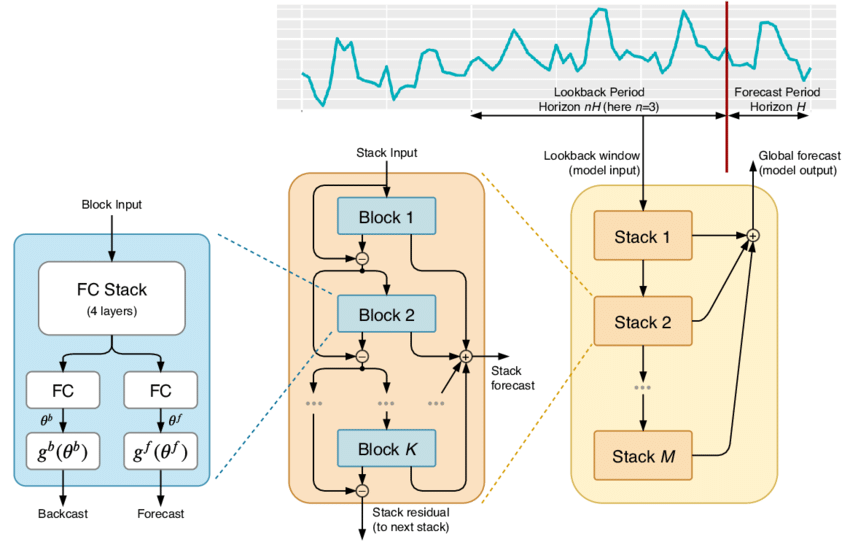
\includegraphics[width=\textwidth]{nbeats}
    \caption{A diagram of the original N-BEATS architecture \cite{oreshkin:nbeats}.}
    \label{fig:nbeats-background}
\end{figure*}

%The recently proposed architecture known as N-BEATS \cite{oreshkin:nbeats} has been shown to achieve state-of-the-art performance on many widely used time series datasets. The N-BEATS architecture is composed of basic blocks (neural networks) that are stacked in a doubly residual manner.

Oreshkin et al. have recently introduced a new architecture for time series forecasting, the \ac{N-BEATS}\cite{oreshkin:nbeats}. The \ac{N-BEATS} architecture is a deep residual model consisting of basic blocks that are stacked in a doubly residual manner. The basic building block of \ac{N-BEATS} is a fully connected structure that initially takes as input a fixed-size lookback period of past values of the target variable and outputs both forecast (estimates of future values) and backcast (estimates of past values) vectors. Blocks are organized into stacks such that the backcast of the current block is subtracted from its input and fed as input to the next block, whereas the forecast vectors from each block are summed up to provide the overall stack forecast. The stacks themselves are chained in a pipeline where the backcast output of one stack is used as input for the next stack. The overall model forecast is then computed by accumulating the forecasts across all the stacks. The \ac{N-BEATS} architecture has been shown to achieve state-of-the-art performance on a variety of widely used time series forecasting datasets \cite{oreshkin:nbeats}. % As such, the \ac{N-BEATS} architecture is a good choice for time series forecasting tasks.

\section{Blood Glucose Prediction}

Providing people with \ac{T1D} the ability to accurately anticipate their impending \ac{BGLs} would be an incredibly helpful and potentially life changing breakthrough. There has been much research with the goal of making this ambition closer to reality with artificial intelligence, specifically machine learning \cite{bunescu:svr_bgl,mirshekarian:bgl_pred,rubin_falcone:nbeats_bgl}. While the end goal of the research in this thesis is not to predict future \ac{BGLs}, there are many parallels between \ac{BGL} prediction and meal and bolus recommendation. \ac{BGL} prediction is essentially the converse of meal or bolus recommendation. \ac{BGL} prediction systems attempt to forecast a \ac{BGL} in the future given information in the present, while meal or bolus recommendation systems use the desired future \ac{BGL} (among other factors) given by the user to recommend a meal or bolus to take in the present in order to reach that \ac{BGL} target. As such, it is important to understand both sides of this problem.

The performance of \ac{BGL} prediction systems has improved due to advances in machine learning, and more specifically deep learning. Neural networks have allowed researchers to bypass the need for expensive, hand-engineered features. Advances in deep learning such as \ac{LSTM} networks \cite{hochreiter:nc97} and the \ac{N-BEATS} architecture \cite{oreshkin:nbeats} have specifically helped improve performance of such systems due to their ability to process temporal \ac{BGL} data. It is important to understand what types of techniques have led to improvement in \ac{BGL} prediction systems, as these same techniques will likely lead to a high level of performance in meal and bolus recommendation systems given the close relationship between the problems.

% Machine learning has been a catalyst in improving the accuracy of \ac{BGL} prediction systems.
In \cite{bunescu:svr_bgl}, a support vector regression model was trained on hand-engineered physiological features based on the raw features extracted from real patient data. This machine learning based approach was shown to outperform three physicians at predicting \ac{BGLs} 30 and 60 minutes into the future. However, creating these hand-engineered features can be time-consuming, expensive, and require the aid of experts in the field of \ac{T1D}. Using deep learning models such as neural networks can eliminate the need for hand-engineered features, as these models can learn relevant features automatically.

In \cite{mirshekarian:bgl_pred}, the authors create a neural network model utilizing the \ac{LSTM} networks described in Section~\ref{section:lstm_background} to predict future \ac{BGLs}. To make these predictions, the models use only raw features from the data, such as a recent history of \ac{BGLs}, insulin, and the carbohydrate counts from recent meals. One of the three training scenarios the authors outlined in the paper, the "what-if" scenario, is a particularly interesting scenario due to its relationship with the meal and bolus recommendation problems. In this scenario, the \ac{BGL} is predicted with the aid of "what-if" events, specifically meals and bolus that occur after the current time, but before the end of the prediction window (the current time + 30 or 60 minutes). 
% Since the models are trained on retroactive data that had already been collected, it is possible to use data from future events to help make the prediction. 
This scenario is useful as it is essentially predicting \ac{BGLs} given some future action intended by the user, such as how many carbs will be in a meal that they plan to eat soon, or how much insulin they plan to bolus in the new few minutes. This could provide people with \ac{T1D} an estimate as to how much a meal or bolus will affect their \ac{BGL} before taking the action. This is essentially the inverse of the research in this thesis, where instead of answering the question "What would my \ac{BGL} be if I eat or bolus this much?", this research aims to answer the question "How much do I need to eat or bolus to get my \ac{BG} to this level?".

%Neural networks are flexible and robust machine learning algorithms that can learn representations of data automatically. Recurrent neural networks have long been the de facto method for processing time-series data in deep learning models. This has been especially true since 1997, when LSTMs were first introduced as a solution to the vanishing gradient problem \cite{hochreiter:nc97}. However, a recently proposed architecture known as N-BEATS \cite{oreshkin:nbeats} has been shown to achieve state-of-the-art performance on many widely used time-series datasets. The N-BEATS architecture, composed of basic blocks (neural networks) that are stacked in a doubly residual manner, has been proven to perform very well on the task of BGL prediction given a few modifications. 

Given the state-of-the-art performance of the \ac{N-BEATS} architecture for time series forecasting tasks Section~\ref{section:nbeats_background}, it is also a natural choice for the \ac{BGL} prediction task. The authors of \cite{rubin_falcone:nbeats_bgl} proposed three important modifications to the original \ac{N-BEATS} architecture to make it better suited for this task. The first, and potentially the most important of these modifications, was the introduction of an \ac{LSTM} into each block to help account for the temporal nature of the blood glucose data. The second proposed modification was the inclusion of additional time series variables, specifically recent carb counts and bolus doses, for each block as context. Without this information, the model would not be able to learn the effects that carbs and insulin have on a subject’s \ac{BGLs}, which would be a missed opportunity for improvement. Finally, the third proposed modification was restructuring the loss function to aid each block in a stack to learn better intermediate representations. With these improvements, the authors achieved top performance on the task of \ac{BGL} prediction \cite{kdh-2020-proceedings}



\section{Insulin Recommendation Systems}

Providing people with \ac{T1D} the ability to preview their future \ac{BGLs} would be of great help in improving the management of their BGLs. However, without the tools to inform a user how to correct their \ac{BGL} if they are predicted to rise too high or sink too low, the usefulness of \ac{BGL} prediction systems is fairly limited. Insulin recommendation systems provide the user with recommendations for how much insulin they should take to lower their \ac{BGL} to the desired target in the near future. There have been a wide range of AI techniques employed to make these insulin recommendation systems such as case-based reasoning \cite{pesl:case_based}, K-nearest-neighbors methods \cite{tyler:knn}, and neural networks \cite{zhu:bolus_drl}. Accuracy is paramount with insulin recommendation systems, as recommendations that are too high or too low can lead to hypoglycemia or hyperglycemia, respectively. Both can cause several long-term complications if not hastily corrected. Therefore, it is critical that insulin recommendation systems be as accurate as possible.

The bolus recommendation system introduced in \cite{pesl:case_based} uses case-based reasoning to provide recommendations for the parameters to be used by a bolus calculator. In this system, cases consist of the meal scenario, the solution (the recommended bolus calculator parameters), and the outcome (the postprandial glucose excursion). When making a recommendation, the system searches through past cases to find a case that is similar to the current situation. If one such case is found, the bolus parameters used in the past case are recommended. If these parameters do not produce the desired outcome (i.e., the subjects postprandial glucose excursion is too high or too low) the original case’s solution is revised by an expert. If no cases similar to the current case are found, a new case is created. This case-based reasoning approach allows the creation of a bolus recommendation system completely personalized to a specific person with \ac{T1D}. However, this system is not learning how meals or boluses affect a person’s \ac{BGL}. It is recalling the bolus recommendations from past instances of similar situations, which have been revised by a clinical expert. While this can lead to very accurate and safe bolus recommendations, it requires an expert to look over the cases and revise the recommendations by hand on a regular basis. This is an expensive and time-consuming task. This also means that when a unique meal scenario that has not been seen before is encountered, the system lacks the ability to make an intelligent prediction.

The authors of \cite{tyler:knn} introduce an insulin recommendation system that provides a user with recommendations on how to improve their \ac{BGLs} through adjustments in their insulin routines. This system uses the K-nearest-neighbors machine learning algorithm to provide up to four (out of 12 possible options) weekly recommendations for adjustments to a user’s insulin dosages. This is done by looking at \ac{BGL}, insulin, and physical activity from the user and classifying which types of recommendations they could benefit from. The goal of this system is to maximize the amount of time that a user spends with a \ac{BGL} in a healthy range while minimizing the amount of time spent in the hypoglycemic range. The system may recommend the user to adjust factors such as their basal insulin rate, their carbs-to-insulin ratio, or their correction factor. While this system offers multiple different types of recommendations, they are adjustments that will have a positive effect on a subject’s \ac{BGL} in a longer-term. As such, it is not as flexible or dynamic as a system that can provide a user with recommendations for real time bolus dosages.

The work in \cite{cappon:bolus_nn} shows that deep learning can be used to personalize the calculation of bolus doses. The authors demonstrated that using a simple feed-forward neural network to calculate bolus doses can outperform other modern methods for \ac{CGM}-based personalized bolus calculators. Neural network models can make recommendations that are specific to an individual by not only considering factors such as insulin on board and target \ac{BGLs}, but also subject-specific parameters such as body weight and insulin sensitivity. While this work shows the usefulness of neural networks for personalizing an individual’s bolus recommendations, this approach does not consider any previous history of \ac{BGLs}, meals, or boluses. Using these features could potentially allow a bolus advisor to make recommendations that are not only personalized for an individual but are personalized for an individual in a specific situation. This would likely result in even better recommendations.

In \cite{zhu:bolus_drl}, the authors proposed a deep reinforcement learning based system for recommending bolus dosages for people with \ac{T1D}. The general approach was to take an action (deliver a bolus) at the time of the meal given the state of the environment (values of various sensors in a glucose control systems) that would maximize the amount of time that a subject’s \ac{BGL} stayed in a healthy range while simultaneously minimizing the amount of time spent in the hypoglycemia range. Since the authors opted to use a reinforcement learning approach, they need an environment in which the models can repeatedly explore various bolus dosages in order to learn a bolus recommendation policy. The ideal environment would be provided by real individuals with \ac{T1D}. However, this would be incredibly unsafe. Even with safety constraints in place, a bad recommendation could force a subject's \ac{BGLs} into a hypoglycemic state. Since training on human subjects is infeasible, the authors used a simulator to train their model, namely the UVA/Padova simulator \cite{dalla_man:simulator}. While simulated data is a more appropriate choice in this situation, it is unclear how well the learned policy would work on data from a real human subject.

The use of insulin recommendation systems can assist people with \ac{T1D} with managing their \ac{BGLs}. There are many different approaches and techniques being used to developing these systems. Similar to \ac{BGL} prediction systems, advances in artificial intelligence continue to enable the creation of improved systems for insulin recommendations. These systems may eventually allow for people with \ac{T1D} to avoid hypoglycemia or hyperglycemia through accurate, safe, and reliable insulin recommendations.

%\section{Contribution}

%The contribution of this thesis is a general neural network architecture that can be trained to make bolus recommendations and meal recommendations. Two architectures were developed and compared on the tasks of bolus and carbohydrate recommendations, an LSTM-based architecture and an N-BEATS-based architecture. The LSTM-based architecture draws inspiration from the architecture introduced in \cite{mirshekarian:bgl_pred} for the task of BGL prediction. The architecture was redesigned to make meal or bolus recommendations using similar input data to that of the original BGL prediction system. The N-BEATS-based architecture is based on the original N-BEATS architecture \cite{oreshkin:nbeats}, and the modified version that was built for the task of BGL prediction \cite{rubin_falcone:nbeats_bgl}. Our N-BEATS-based architecture makes additions to these architectures which make them better suited for the tasks of bolus and meal recommendations. Both architectures are trained on the OhioT1DM dataset \cite{marling:ohiot1dm}, which contains data from real people with T1D. The goal of this research is to use real-patient data and proven BGL prediction architectures to create accurate, personalized bolus and meal recommendation systems.

\chapter{Deep Learning Models for Carbohydrate and Bolus Recommendations}
\label{chapter:models}

This chapter will expand on the general problem description from Section~\ref{section:objective} and introduce in detail the situations commonly encountered in diabetes self-management that could benefit from the research reported in this thesis. Two neural network models will be introduced, as well as a two baseline models, and all will be evaluated extensively on the tasks of carbohydrate and bolus recommendation using examples extracted from the OhioT1DM dataset.

\section{Recommendation Scenarios}
\label{sec:scenarios}

It is assumed that blood glucose levels are measured at 5 minute intervals through a \ac{CGM} system. It is also assumed that discrete deliveries of insulin (boluses) and continuous infusions of insulin (basal rates) are recorded. Subjects provide the timing of meals and estimates of the number of grams of carbohydrate in each meal. Given the available data up to and including the present (time $t$), the system aims to estimate how much a person should eat or bolus 10 minutes from now (time $t+10$) such that their blood glucose will reach a target level $\tau$ minutes after that action (time $t + 10 + \tau$). A system that computes these estimates could then be used in the following three recommendation scenarios:
\begin{enumerate}
    \item {\bf Carbohydrate Recommendations}: Estimate the amount of carbohydrate $C_{t+10}$ to have in a meal in order to achieve a target \ac{BG} value $G_{t+10+\tau}$.
    \item {\bf Bolus Recommendations}: Estimate the amount of insulin $B_{t+10}$ to deliver with a bolus in order to achieve a target \ac{BG} value $G_{t+10+\tau}$.
    \item {\bf Bolus Recommendations given Carbohydrates}: Expecting that a meal with $C_{t+20}$ grams of carbohydrate will be consumed 20 minutes from now, estimate the amount of insulin $B_{t+10}$ to deliver with a bolus 10 minutes before the meal in order to achieve a target \ac{BG} value $G_{t+10+\tau}$.
\end{enumerate}
These recommendation scenarios were designed to align with decision-making situations commonly encountered by people with type 1 diabetes. In particular, the corresponding recommendation systems would help an individual to estimate how much to eat or bolus for the purpose of raising or lowering their \ac{BGL} (scenarios 1 and 2), as well as how much to bolus for a planned meal (scenario 3). 

%\textcolor{blue}{While all three of these scenarios are useful, there are two specific subsets of these cases that are of particular interest. The carbohydrate recommendation scenario evaluated only on meals that do not have an associated boluses is especially relevant because these are the situations where a subject presumably ate a snack specifically to raise their BGL. The bolus recommendation scenario trained and evaluated exclusively on inertial examples also is particularly useful, as the boluses in these examples are not taken with a meal. This means that these boluses were likely taken to lower the subject's BGL. These two specific scenarios are the most interesting in practice. However, they both are fairly uncommon in the particular dataset that we used.}

%In the following Section~\ref{sec:models}, \textcolor{blue}{a number of baseline models and neural architectures are described}, all implementing the three types of recommendations. The neural architectures use Long Short-Term Memory (LSTM) networks either in a standalone prediction model (Section~\ref{sec:lstm}) or integrated as basic repeating blocks in a deep residual network (Section~\ref{sec:nbeats}). The models are trained on examples extracted from the OhioT1DM dataset~\cite{ohiot1dm:marling:kdh18}, as explained in Chapter~\ref{chapter:data}. Ideally, to match the intended use of these recommendations in practice, training examples should not have any extra meals or boluses in the prediction window $[t, t + 10 + \tau]$. Following the terminology from \cite{mirshekarian:bgl_pred}, \textcolor{blue}{these examples are called {\it inertial} examples.} However, to benefit from a larger number of training examples, \textcolor{blue}{models are also trained and evaluated on a more general class of {\it unrestricted} examples}, in which other bolus or meal events are allowed to appear in the prediction window. Correspondingly, experimental results for inertial vs. unrestricted examples are presented in Section~\ref{sec:results}. 

%The paper ends in Section~\ref{sec:conclusion} with concluding remarks and ideas for future work.
% In Section~\ref{sec:results} we show the extent to which models trained on the larger set of unrestricted examples transfer to inertial examples.

%Ideally, all examples of the above prediction scenarios in the data would not have any extra meals or boluses in the prediction window between $t$ and $t+10+\tau$. These events would not be known in practice since they are in the future. However, if only examples without these such events were used, it would limit the number of examples that can be extracted from the data. For this reason, examples are separated into 2 classes based on the following criteria:

%\begin{enumerate}
%    \item {\bf Class $\mathbf{C_{1}}$} examples do not contain events in the prediction window $(t, t+10+\tau)$ other than the meal or bolus that is to be predicted. When the bolus given carbohydrates prediction scenario is used, the meal that follows the bolus is also allowed in a C$_1$ example. This class of example most closely represents the situations in which the system would be used in practice. However, these examples are somewhat limited, especially for the bolus prediction scenario.
%    \item {\bf Class $\mathbf{C_{2}}$} is more general and allows other events to be in the prediction window $(t, t+10+\tau)$. This class yields a higher number of examples, but resembles a real world situation less than C$_1$, since there are unknown events past the present time $t$. Because of this, a more complex model is required to process C$_2$ examples.
%\end{enumerate}

%Using both classes of examples allows us to see how well the models do on examples similar to real world use, C$_1$, as well as how well the models do with the maximum number of possible examples in the dataset with C$_2$.


\section{Recommendation Models}
\label{sec:models}

In the following sections, a number of baseline models and neural architectures are described, all implementing the three types of recommendations. The neural architectures use \ac{LSTM} networks either in a standalone prediction model (Section~\ref{sec:lstm}) or integrated as basic repeating blocks in a deep residual network (Section~\ref{sec:nbeats}). The models are trained on examples extracted from the OhioT1DM dataset~\cite{ohiot1dm:marling:kdh18}, as explained in Chapter~\ref{chapter:data}. Ideally, to match the intended use of the recommendation scenarios from Section~\ref{sec:scenarios}, training examples should not have any extra meals or boluses in the prediction window $[t, t + 10 + \tau]$. Following the terminology from \cite{mirshekarian:bgl_pred}, these examples are called {\it inertial} examples. However, to benefit from a larger number of training examples, models are also trained and evaluated on a more general class of {\it unrestricted} examples, in which other bolus or meal events are allowed to appear in the prediction window. Correspondingly, experimental results for both inertial vs. unrestricted examples are presented in Section~\ref{sec:results}.

\subsection{Baseline Models}
Given training data containing time series of blood glucose levels, meals with their carbohydrate intake, and boluses with their corresponding insulin dosages, two baselines are defined as follows:
\begin{enumerate}
    \item {\bf Global average}: 
    For the carbohydrate recommendation scenario, the average number $\mu$ of carbs over all of the meals in the subject's training data is computed and used as the estimate for all future predictions for that subject, irrespective of the context of the example. Analogously, for the bolus and bolus given carbs recommendation scenarios, $\mu$ is the average amount of insulin dosage over all boluses in the subject's training data. This is a fairly simple baseline, as it predicts the same average value for every test example for a particular subject.
    
    %Compute the average number of carbs over all of the meals in the subject's training data, and use this average $\mu$ as the estimate for all future meals, irrespective of context. This is a fairly simple baseline, as it predicts the same value for every example.
    \item {\bf \ac{ToD} average}: In this \ac{ToD} dependent baseline, an average number of carbs or an average amount of bolus insulin is computed for each of the following five time windows during a day:
	\begin{itemize}
		\item 12am-6am: $\mu_1$ = early breakfast / late snacks.
		\item 6am-10am: $\mu_2$ = breakfast.
		\item 10am-2pm: $\mu_3$ = lunch.
		\item 2pm-6pm: $\mu_4$ = dinner.
		\item 6pm-12am: $\mu_5$ = late dinner / post-dinner snacks.
	\end{itemize}
    The average for each \ac{ToD} interval is calculated over all of the meals or boluses appearing in the corresponding time frame in the subject's training data. At test time, to make a recommendation for time $t+10$, the \ac{ToD} interval that contains $t+10$ is determined and the corresponding \ac{ToD} average is used as the recommendation.
\end{enumerate}
Given sufficient historical data, the \ac{ToD} baseline is expected to perform well for individuals who tend to eat very consistently and have regular diets. However, it is expected to perform poorly for individuals who have a lot of variation in their diets.

% For the bolus given carbs recommendation scenario, one might have also considered a bolus calculator `baseline', for which insulin dosages would be computed using the actual bolus calculator employed by the subjects in the OhioT1DM dataset every time they had a meal. However, assuming subjects had perfect adherence to using the bolus calculator, this `baseline' would coincide with the ground truth every time, making it inappropriate as a baseline.

\begin{figure*}[t]
    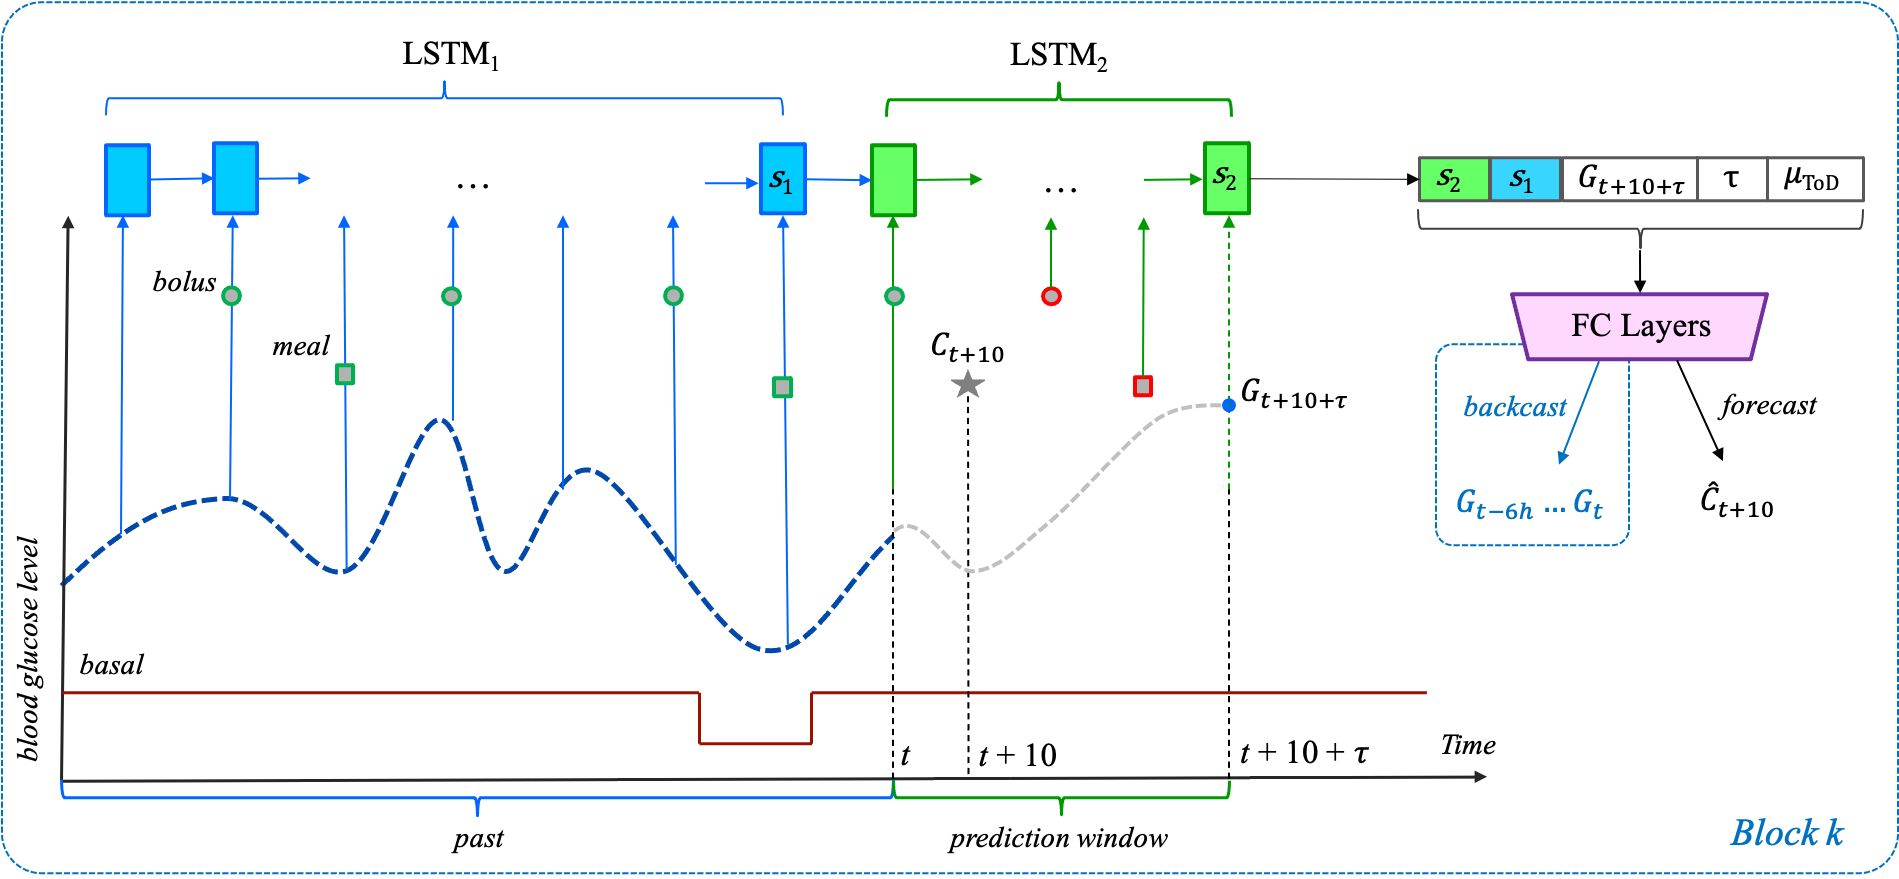
\includegraphics[width=\textwidth]{carbs-block}
    \caption{The general neural network architecture for the carbohydrate recommendation scenario. The dashed blue line in the graph represents a subject's \ac{BGL}, while the solid brown line represents the basal rate of insulin. The gray star represents the meal at time $t+10$. The other meals are represented by squares, and boluses are represented by circles. Meals and boluses with a red outline cannot appear in {\it inertial} examples, but are allowed in {\it unrestricted} examples. The blue units in $\text{LSTM}_{1}$ receive input from different time steps in the past. The green units in $\text{LSTM}_{2}$ receive input from the prediction window. The purple trapezoid represents the 5 fully connected layers, whereas the output node at the end computes the prediction.}
    \label{fig:carbs}
\end{figure*}

\begin{figure*}[t]
    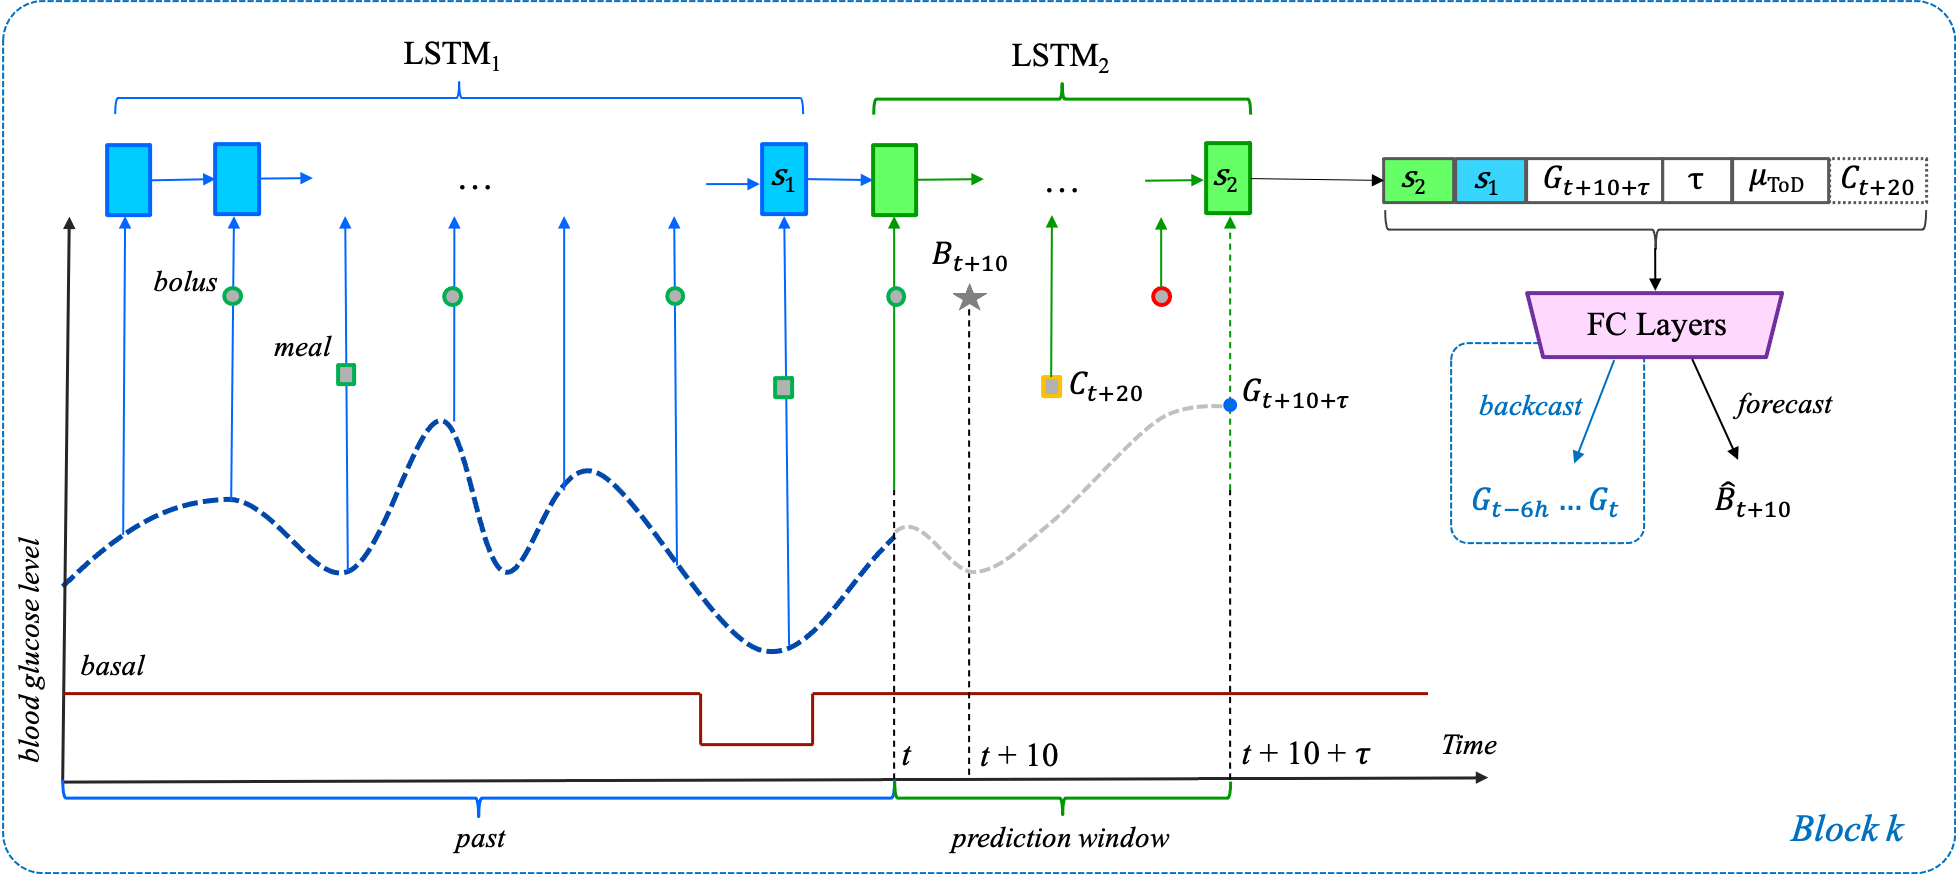
\includegraphics[width=\textwidth]{bolus-block}
    \caption{The general neural network architecture for the bolus and bolus given carbs recommendation scenarios. The architecture itself is similar to that shown in Figure~\ref{fig:carbs}. The gray star now represents the bolus at time $t+10$. For the bolus recommendation scenario, the events outlined in red or orange are not allowed in {\it inertial} examples.  However, in the bolus given carbs scenario, the meal event $C_{t+20}$ shown with the yellow outline is an important part of each example, be it inertial or unrestricted. As such, in this scenario, the dashed $C_{t+20}$ becomes part of the input to the FCN.}
    \label{fig:bolus}
\end{figure*}

\begin{figure*}[t]
    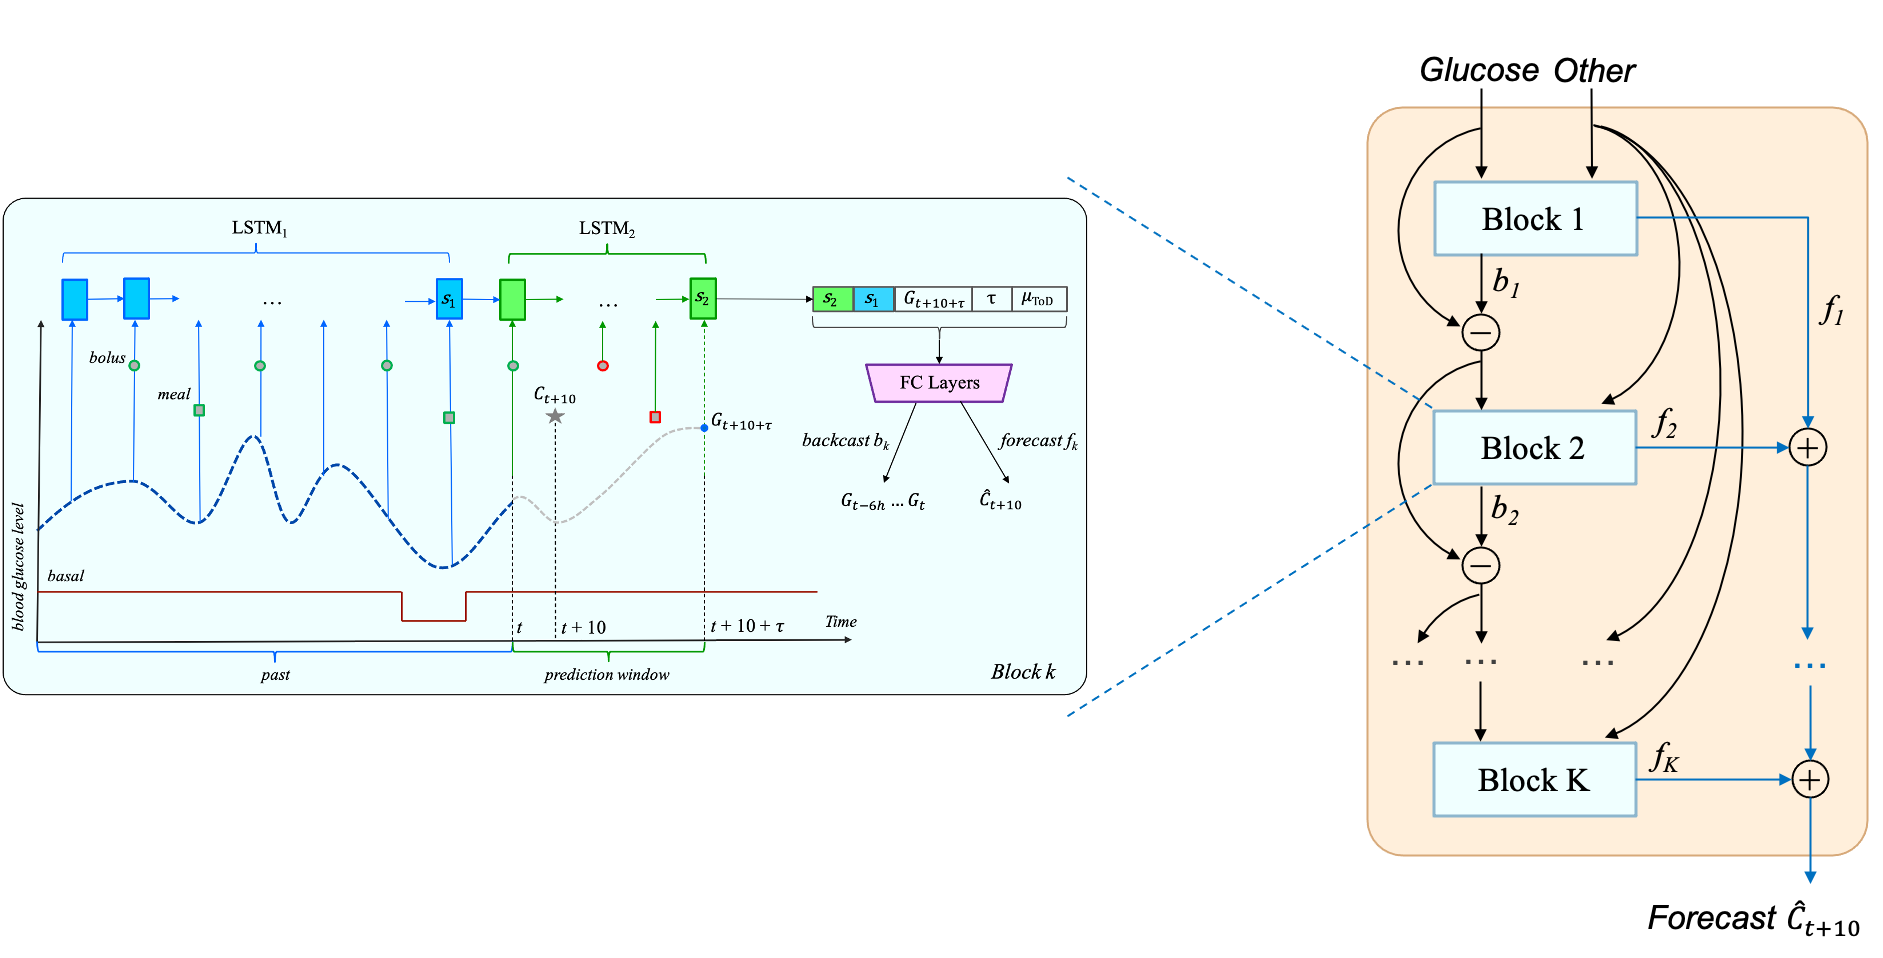
\includegraphics[width=\textwidth]{carbs-nbeats}
    \caption{The N-BEATS inspired deep residual architecture for carbohydrate recommendation. A similar architecture is used for bolus and bolus given carbs recommendations.}
    \label{fig:nbeats}
\end{figure*}


\subsection{LSTM Architectures}
\label{sec:lstm}

While simple to compute and use at test time, the two baselines are likely to give suboptimal performance, as their predictions ignore the history of \ac{BGL} values, insulin (boluses and basal rates), and meals, all of which could significantly modulate the effect a future meal and/or bolus might have on the \ac{BGL}. To utilize this information, the general \ac{LSTM}-based network architectures shown in Figure~\ref{fig:carbs} for carb recommendation and Figure~\ref{fig:bolus} for bolus recommendation were developed. The first component in each architecture is a recurrent neural network instantiated using \ac{LSTM} cells \cite{hochreiter:nc97}, which is run over the previous 6 hours of data, up to and including the present time $t$. At each time step (every 5 minutes), this LSTM$_1$ network takes as input the \ac{BGL}, the carbs, and the insulin dosages recorded at that time step. While sufficient for processing {\it inertial} examples, the same \ac{LSTM} cannot be used to process events that may appear in the prediction window $(t, t+10+\tau)$ of {\it unrestricted} examples, because \ac{BGL} values are not available in the future. Therefore, when training on unrestricted examples, the final state computed by the LSTM$_1$ model at time $t$ is projected using a linear transformation and used as the initial state for a second \ac{LSTM} network, LSTM$_2$, that is run over all the time steps in the prediction window $(t, t+10+\tau)$. The final state computed by LSTM$_1$ (for inertial examples) is appended to the final state computed by LSTM$_2$ (for unrestricted examples) and is then used as input to a \ac{FCN} whose output node computes an estimate of the carbs or bolus insulin at time $t+10$. In addition to the \ac{LSTM} final state(s), the input to the \ac{N-BEATS} contains the following features:
\begin{itemize}
    \item The target blood glucose level $\tau+10$ minutes into the future, i.e., $G_{t + 10 + \tau}$.
    \item The prediction horizon $\tau$.
    \item The \ac{ToD} average for the time frame that contains $t+10$.
    \item For the bolus given carbs scenario only, the planned amount $C_{t + 20}$ of carbohydrate becomes part of the input, too.
\end{itemize}
Each \ac{LSTM} uses vectors of size 32 for the states and gates, whereas the \ac{N-BEATS} is built with up to 5 hidden layers, each consisting of 64 ReLU neurons, and one linear output node. Note that by using the final state of LSTM$_1$  to initialize LSTM$_2$, the latter's final state should theoretically be able to capture any useful information that is represented in the final state of LSTM$_1$, which may call into question the utility of concatenating the two final states. This architectural decision is nevertheless supported empirically through evaluations on the validation data, which show improvements in prediction performance when both states are used (Section~\ref{sec:development}).

\subsection{Deep Residual Networks}
\label{sec:nbeats}

%\citet{oreshkin:nbeats} have recently introduced a new architecture for time series forecasting, the Neural Basis Expansion for Interpretable Time-Series Forecasting (N-BEATS). The basic building {\it block} of N-BEATS is a fully connected structure that initially takes as input a fixed-size {\it lookback period} of past values of the target variable and outputs both {\it forecast} (estimates of future values) and {\it backcast} (estimates of past values) vectors. Blocks are organized into {\it stacks} such that the backcast of the current block is subtracted from its input and fed as input to the next block, whereas the forecast vectors from each block are summed up to provide the overall {\it stack forecast}. The stacks themselves are chained in a pipeline where the backcast output of one stack is used as input for the next stack. The overall model forecast is then computed by accumulating the forecasts across all the stacks.

The \ac{N-BEATS} architecture described in Section~\ref{section:nbeats_background} has been shown to obtain state-of-the-art performance on a wide range of time series prediction tasks \cite{oreshkin:nbeats}, which suggests that it can serve as a model of choice for \ac{BGL} prediction, too. However, in \ac{BGL} prediction, time series of variables other then the primary blood glucose are also available. Correspondingly, the Rubin-Falcone et al. \cite{rubin_falcone:nbeats_bgl} changed the \ac{N-BEATS} block architecture to also use as input secondary, sparse variables such as meals and bolus insulin, while still backcasting only on the primary forecasting variable, blood glucose. To account for the temporal nature of the input, the fully connected structure of the basic \ac{N-BEATS} block was replaced with \ac{LSTM} networks, followed by one fully connected layer whose output was split into the backcast and forecast vector. Additional per-block forecast and backcast loss terms were also added to provide more supervision.

The deep residual network from \cite{rubin_falcone:nbeats_bgl} has been adapted to perform carb or bolus recommendations by using the \ac{LSTM}-based architecture from Section~\ref{sec:lstm} to instantiate each block in the stack, as shown in Figure~\ref{fig:nbeats}. Compared to the architecture from \cite{rubin_falcone:nbeats_bgl}, the most significant differences are:
\begin{enumerate}
    \item The use of a chain of two \ac{LSTM} networks in each block.
    \item The inclusion of additional inputs to the fully connected layers, i.e. the target \ac{BG} level, the time horizon, and the \ac{ToD} average.
    \item While backcasting is still done for blood glucose, forecasting is done for carbs or bolus, depending on the recommendation scenario.
\end{enumerate}
While Oreshkin et al. \cite{oreshkin:nbeats} used 30 blocks and Rubin-Falcone et al. \cite{rubin_falcone:nbeats_bgl} used 10 blocks, the validation experiments for the recommendation tasks showed that the most effective deep residual architecture uses only up to 5 blocks, depending on the recommendation scenario (Section~\ref{sec:development}).

\chapter{The OhioT1DM Dataset for Recommendation Examples}
\label{chapter:data}

%\section{}
%\label{sec:dataset}

To evaluate the proposed recommendation models, training and test examples are created using data collected from 12 subjects with type 1 diabetes that is distributed with the OhioT1DM dataset~\cite{ohiot1dm:marling:kdh20}. The 12 subjects are partitioned in two subsets as follows:
\begin{enumerate}
    \item {\bf OhioT1DM 2018}: This is the first part of the dataset, containing data collected from 6 patients. It was used for the 2018 \ac{BGLP} challenge \cite{kdh-2018-proceedings}.
    \item {\bf OhioT1DM 2020}: This is the second part of the dataset, containing data collected from 6 additional patients. It was used for the 2020 \ac{BGLP} challenge \cite{kdh-2020-proceedings}.
\end{enumerate}
Time series containing the basal rate of insulin, boluses, meals, and \ac{BGL} readings were collected over 8 weeks, although the exact number of days varies from subject to subject. 
Insulin and \ac{BGL} data was automatically recorded by each subject's insulin pump.  Meal data was collected in two different ways.  Subjects self reported meal times and estimated carbs via a smartphone interface.  Subjects also entered estimated carbs into a bolus calculator when bolusing for meals, and this data was recorded by the insulin pump.

\section{The Bolus Wizard}
\label{sec:bw}

To determine their insulin dosages, the subjects in the OhioT1DM study used a bolus calculator, or \ac{BW}, which was integrated in their insulin pumps.  They used it to calculate the bolus amount before each meal as well as when using a bolus to correct for hyperglycemia.  To use the \ac{BW}, a subject enters their current blood glucose level and, if eating, their estimated number of grams of carbohydrate.  To calculate a recommended insulin dosage, the \ac{BW} uses this input from the subject, plus the amount of active insulin the subject already has in their system, along with the following three pre-programmed, patient-specific parameters:
\begin{enumerate}
    \item The carb ratio, which indicates the number of grams of carbohydrate that are covered by a unit of insulin.
    \item The insulin sensitivity, which tells how much a unit of insulin is expected to lower the subject's blood glucose level.
    \item The target blood glucose range, which defines an individual's lower and upper boundaries for optimal blood glucose control.
\end{enumerate}
All three parameters may vary, for the same individual, throughout the day and over time\footnote{\url{https://www.medtronicdiabetes.com/loop-blog/4-features-of-the-bolus-wizard}}. Given this input and these parameters, the \ac{BW} calculates the amount of insulin the subject should take to maintain or achieve a blood glucose level within their target range. The calculation is displayed to the subject as a recommendation, which the subject may then accept or override.

Based on the inputs and the patient-specific parameters described above, the \ac{BW} uses a deterministic formula to calculate the bolus amount before each meal. As such, when trained in the bolus given carbs recommendation scenario, there is the risk that the deep learning models introduced in Section~\ref{sec:models} might simply learn to reproduce this deterministic dependency between bolus and carbs, while ignoring the target \ac{BG} level that is used as input. However, this is not the case in our experimental settings, for the following reasons:
\begin{itemize}
    \item The machine learning models do not have access to any of the three patient-specific parameters above, which can change throughout the day and over time, and which are set based on advice from a health care professional.
    \item The \ac{BW} uses a fixed target \ac{BG} range depending on the time of day, whereas the target in the recommendation scenarios is a more specific \ac{BG} level, to be achieved at a specific time in the near future.
    \item The amount of insulin calculated by the \ac{BW} is only a recommendation, which is often overridden by subjects. An analysis of the OhioT1DM dataset was conducted in order to count the number of times the amount of insulin that was actually delivered was different from the BW recommendation. The analysis revealed that, of all the times that the \ac{BW} was used, its recommendation was overridden for about a fifth of the boluses. Furthermore, there are subjects in the dataset who often did not use the \ac{BW} (540 and 567), or who 
    chose to not use the \ac{BW} at all (596).
\end{itemize}
Therefore, the machine learning models will have to go beyond using solely the carbohydrate amount in the intended meal. In order to fit the bolus recommendation examples, they will need to learn the impact that a bolus has on the target \ac{BG} level for the specified prediction horizon, taking into account the amount of carbohydrate in the meal as well as the history of carbs, insulin, and \ac{BG} levels. This data driven approach to bolus recommendation relieves the physician from the cognitively demanding task of regularly updating parameters such as the carb ratio and the insulin sensitivity, which often requires multiple fine tuning steps. In contrast, any relevant signal that is conveyed through the carb ratio and insulin sensitivity is expected to be learned by the machine learning models from the data.


\section{Pre-processing of Meals and BG Levels}
\label{sec:pre-processing}

While exploring the data, it was observed that self-reported meals and their associated boluses were in unexpected temporal positions relative to each other. For many meals, patients recorded a timestamp in the smartphone interface that preceded the corresponding bolus timestamp recorded in the insulin pump. This was contrary to what was recommended to the subjects by their physicians, which was to bolus shortly before the meal, and no more than 15 minutes prior to the meal. This discrepancy is likely due to subjects reporting incorrect meal times in the smartphone interface.

To correct the meal events, the data provided to the \ac{BW} was used in a pre-processing step that changed the timestamp of each meal associated with a bolus to be exactly 10 minutes after that bolus. For these meals, the number of carbs provided to the \ac{BW} was used, which is likely to be more accurate than the estimate provided by the subject through the smartphone interface. To determine if the self-reported meal event was associated with a bolus having non-zero carb input, the meal that was closest to the bolus was searched within one hour before or after it. In case there were two meals that were equally close to the bolus, the one for which the number of carbs reported in the smartphone interface was closest to the number of carbs entered into the \ac{BW} was selected. If no self-reported meal was found within one hour of the bolus, it was assumed that the subject forgot to log their meal on the smartphone interface. As such, a meal was added 10 minutes after the bolus, using the amount of carbs specified in the \ac{BW} for that bolus. Ablation results reported in Section~\ref{sec:pre-evaluation} show that this pre-processing of meal events leads to significantly more accurate predictions, which further justifies the pre-processing.

All gaps in \ac{BGL} data are filled in with linearly interpolated values. However, examples that meet any of the following criteria are filtered out:
\begin{enumerate}
    \item The \ac{BGL} target is interpolated.
    \item The \ac{BGL} at present time $t$ is interpolated.
    \item There are more than 2 interpolated \ac{BGL} measurements in the one hour of data prior to time $t$.
    \item There are more than 12 interpolated \ac{BGL} measurements in the 6 hours of data prior to time $t$.
\end{enumerate}



\section{Mapping Prototypical Recommendation Scenarios to Datasets}
\label{sec:mapping}

According to the definition given in Section~\ref{sec:scenarios}, the carbohydrate recommendation scenario refers to estimating the amount of carbohydrate $C_{t+10}$ to have in a meal in order to achieve a target \ac{BG} value $G_{t+10+\tau}$. This is done by using the history of data up to and including the present time $t$. However, many carbohydrate intake events $C_{t+10}$ are regular meals, which means that they are preceded by a bolus event at time $t$. Since in the carbohydrate recommendation scenario, the cases where the subject eats in order to correct or prevent hypoglycemia are particularly of interest, two separate datasets for carbohydrate prediction were created:
\begin{enumerate}
    \item Carbs$^{(\pm b)}$: this will contain examples for all carbohydrate intake events, with $(+b)$ or without $(-b)$ an associated bolus.
    \item Carbs$^{(-b)}$: this will contain examples only for carbohydrate intake events without $(-b)$ an associated bolus.
\end{enumerate}
Most of the Carbs$^{(-b)}$ examples are expected to happen in one of three scenarios: (1) when correcting for hypoglycemia; (2) before exercising; and (3) when having a bedtime snack to prevent nocturnal hypoglycemia. Given that they are only a small portion of the overall carbohydrate events, Section~\ref{sec:results} presents the results for both Carbs$^{(\pm b)}$ and Carbs$^{(-b)}$ recommendation scenarios.

Furthermore, mirroring the two bolus recommendation scenarios introduced in Section~\ref{sec:scenarios}, the following dataset notation is used:
\begin{enumerate}
    \item Bolus$^{(\pm c)}$: this will contain examples for all bolus events, with $(+c)$ or without $(-c)$ an associated carbohydrate intake.
    \item Bolus$^{(+c)}$: this will contain examples only for the bolus events with $(+c)$ an associated carbohydrate intake.
\end{enumerate}
The three major recommendation scenarios introduced in Section~\ref{sec:scenarios} can then be mapped to the corresponding datasets as follows:
\begin{enumerate}
    \item {\bf Carbohydrate Recommendations}: Estimate the amount of carbohydrate $C_{t+10}$ to have in a meal in order to achieve a target \ac{BG} value $G_{t+10+\tau}$.
    \begin{itemize}
        \item Carbs$^{(-b)}$, inertial: this reflects the prototypical scenario where a carbohydrate intake is recommended to correct or prevent hypoglycemia.
    \end{itemize}
    \item {\bf Bolus Recommendations}: Estimate the amount of insulin $B_{t+10}$ to deliver with a bolus in order to achieve a target \ac{BG} value $G_{t+10+\tau}$.
    \begin{itemize}
        \item Bolus$^{(\pm c)}$, inertial: this reflects the prototypical scenario where a bolus is recommended to correct or prevent hyperglycemia. Because in the inertial case a carb event cannot appear after the bolus, this could also be denoted as Bolus$^{(-c)}$.
    \end{itemize}
    \item {\bf Bolus Recommendations given Carbohydrates}: Expecting that a meal with $C_{t+20}$ grams of carbohydrate will be consumed 20 minutes from now, estimate the amount of insulin $B_{t+10}$ to deliver with a bolus 10 minutes before the meal in order to achieve a target \ac{BG} value $G_{t+10+\tau}$.
    \begin{itemize}
        \item Bolus$^{(+c)}$, inertial: this reflects the prototypical scenario where a bolus is recommended before a meal.
    \end{itemize}
\end{enumerate}


\section{Carbohydrate and Bolus Statistics}
\label{sec:statistics}

Table~\ref{tab:meals} shows the number of carbohydrate events in each subject's pre-processed data, together with the minimum, maximum, median, average, and standard deviation for the number of carbs per meal. Overall, the average number of carbs per meal is between 22 and 69, with the exception of subjects 570 and 544 whose meal averages and standard deviations are significantly larger. 
Table~\ref{tab:boluses} shows similar statistics for boluses and their dosages, expressed in units of insulin.
Overall, the number of boluses is more variable than the number of meals. There is also a fairly wide range of average bolus values in the data, with subject 567 having a much higher average than other subjects. It is also interesting to note that subject 570, who had the largest average carbs per meal, had more than twice the number of boluses than any other subject while at the same time having the lowest average bolus. Subject 570 also used many dual boluses, which were not used as prediction labels because the scope of the project covers only recommendations for regular boluses.

\begin{table}[t]\setlength{\tabcolsep}{4pt}
\begin{center}
\caption{Per subject and total meal and carbohydrate per meal statistics: Minimum, Maximum, Median, Average, and Standard Deviation (StdDev). Carbs$^{(\pm b)}$ refers to all carbohydrate intake events; Carbs$^{(-b)}$ refers to carbohydrate intakes without a bolus. Statistics are shown for the 2018 subset, the 2020 subset, and for the entire OhioT1DM dataset.}
\label{tab:meals}
\small
\begin{tabular}{|crr|rrrrc|}
    \cline{4-8}
    \multicolumn{3}{c}{} & \multicolumn{5}{|c|}{Carbs Per Meal}\\
	\hline
	Subject & \multicolumn{1}{c}{Carbs$^{(\pm b)}$} & \multicolumn{1}{c|}{Carbs$^{(-b)}$} & \multicolumn{1}{c}{Minimum} & \multicolumn{1}{c}{Maximum}
	& \multicolumn{1}{c}{Median} & \multicolumn{1}{c}{Average} & StdDev\\
	\hline
	559 & 215 & 83 & 8.0 & 75.0 & 30.0 & 35.5 & 15.5\\
    563 & 225 & 28 & 5.0 & 84.0 & 31.0 & 33.8 & 18.0\\
    570 & 174 & 39 & 5.0 & 200.0 & 115.0 & 106.1 & 41.5\\
	575 & 297 & 122 & 1.0 & 110.0 & 40.0 & 40.0 & 22.0\\
	588 & 268 & 73 & 2.0 & 60.0 & 20.0 & 22.7 & 14.6\\
	591 & 264 & 60 & 3.0 & 77.0 & 28.0 & 31.5 & 14.1\\
	\hline
	2018 Total & 1443 & 405 & 1.0 & 200.0 & 33.0 & 41.5 & 32.7\\
	\hline
	540 & 234 & 14 & 1.0 & 110.0 & 40.0 & 50.2 & 29.8\\
	544 & 206 & 41 & 1.0 & 175.0 & 60.0 & 68.7 & 36.3\\
	552 & 271 & 25 & 3.0 & 135.0 & 26.0 & 36.7 & 29.3\\
	567 & 207 & 5 & 20.0 & 140.0 & 67.0 & 67.0 & 21.5\\
	584 & 233 & 44 & 15.0 & 78.0 & 60.0 & 54.6 & 11.6\\
	596 & 300 & 277 & 1.0 & 64.0 & 25.0 & 25.1 & 14.0\\
	\hline
	2020 Total & 1451 & 406 & 1.0 & 175.0 & 42.0 & 48.2 & 29.5\\
	\hline
	Combined Total & 2894 & 811 & 1.0 & 200.0 & 39.0 & 44.9 & 31.3\\
	\hline
\end{tabular}
\end{center}
\end{table}

\begin{table}[t]\setlength{\tabcolsep}{4pt}
\begin{center}
\caption{Per subject and total boluses and insulin units statistics: Minimum, Maximum, Median, Average, and Standard Deviation (StdDev). Bolus$^{(\pm c)}$ refers to all bolus events; Bolus$^{(+c)}$ refers to bolus events associated with a meal. Statistics are shown for the 2018 subset, the 2020 subset, and for the entire OhioT1DM dataset.}
\label{tab:boluses}
\small
\begin{tabular}{|crr|rrrrc|}
    \cline{4-8}
    \multicolumn{3}{c|}{} & \multicolumn{5}{c|}{Insulin Per Bolus}\\
	\hline
	Subject & \multicolumn{1}{c}{Bolus$^{(\pm c)}$} & \multicolumn{1}{c|}{Bolus$^{(+c)}$}
	& \multicolumn{1}{c}{Minimum} & \multicolumn{1}{c}{Maximum} & \multicolumn{1}{c}{Median} & \multicolumn{1}{c}{Average} & StdDev\\
	\hline
	559 & 186 & 132 & 0.1 & 9.3 & 3.6 & 3.7 & 1.9\\
    563 & 424 & 197 & 0.1 & 24.7 & 7.8 & 8.0 & 4.2\\
    570 & 1,345 & 132 & 0.2 & 12.1 & 1.3 & 1.8 & 2.1\\
	575 & 271 & 175 & 0.1 & 12.8 & 4.4 & 4.1 & 3.0\\
	588 & 221 & 195 & 0.4 & 10.0 & 3.5 & 4.3 & 2.3\\
	591 & 331 & 204 & 0.1 & 9.4 & 2.9 & 3.1 & 1.8\\
	\hline
	2018 Total & 2,758 & 1,035 & 0.1 & 24.7 & 1.9 & 3.5 & 3.4\\
	\hline
	540 & 521 & 220 & 0.1 & 11.4 & 2.0 & 3.0 & 2.8\\
	544 & 264 & 149 & 0.7 & 22.5 & 5.0 & 6.5 & 4.9\\
	552 & 426 & 246 & 0.1 & 16.0 & 2.8 & 3.9 & 3.3\\
	567 & 366 & 202 & 0.2 & 25.0 & 11.4 & 12.0 & 5.8\\
	584 & 311 & 188 & 0.1 & 16.2 & 9.1 & 7.3 & 3.1\\
	596 & 230 & 0 & 0.2 & 7.6 & 3.3 & 3.0 & 1.5\\
	\hline
	2020 Total & 2,118 & 1,169 & 0.1 & 25.0 & 4.0 & 5.8 & 5.0\\
	\hline
	Combined Total & 4,876 & 2,204 & 0.1 & 25.0 & 2.9 & 4.5 & 4.3\\
	\hline
\end{tabular}
\end{center}
\end{table}

\section{From Meals and Bolus Events to Recommendation Examples}
\label{sec:examples}

In all recommendation scenarios, the prediction window ranges between the present time $t$ and the prediction horizon $t + 10 + \tau$. For the carbohydrate or bolus recommendation scenarios, the meal or the bolus is assumed to occur at time $t +10$. For the bolus given carbs scenario, the bolus occurs at time $t+10$ and is followed by a meal at time $t+20$, which matches the pre-processing of the meal data. For evaluation purposes, $\tau$ is set to values between 30 and 90 minutes with a step of 5 minutes, i.e, $\tau \in \{30, 35, 40, ..., 90\}$ for a total of 13 different values. As such, each meal/bolus event in the data results in 13 recommendation examples, one example for each value of $\tau$. While all 13 examples use the same value for the prediction label, e.g., $B_{t + 10}$ for bolus prediction, they will differ in terms of the target \ac{BG} feature $G_{t + 10 + \tau}$ and the $\tau$ feature, both used directly as input to the FC layers in the architectures shown in Figures~\ref{fig:carbs} and~\ref{fig:bolus}. For the bolus given carbs scenario, the 13 examples are only created when there is a meal that had a bolus delivered 10 minutes prior. Due to the way the data is pre-processed, it is guaranteed that if a meal had a bolus associated with it, the bolus will be exactly 10 minutes before the meal. 

Table \ref{tab:c1_examples} shows the number of {\it inertial} examples for 5 prediction horizons, as well as the total over all 13 possible prediction horizons. Table \ref{tab:c2_examples} shows the number of {\it unrestricted} examples. Since the same number of unrestricted examples are available for every prediction horizon, only the totals are shown. The only exceptions would be if an event was near the end of a subject's data and the prediction horizon $t+10+\tau$ goes past the end of the dataset for some value of $\tau$.

\begin{table}[ht]\setlength{\tabcolsep}{4pt}
\begin{center}
\caption{{\it Inertial} ({\it I}) examples by recommendation scenario and prediction horizon. Carbs$^{(\pm b)}$ refers to all carbohydrate intake events; Carbs$^{(-b)}$ refers to carbohydrate intakes without a bolus.}
\label{tab:c1_examples}
\small
\begin{tabular}{|l|rrrr|rrrr|}
    \cline{2-9}
    \multicolumn{1}{c}{}& \multicolumn{4}{|c|}{Carbs$^{(\pm b)}$ recommendation} & \multicolumn{4}{c|}{Carbs$^{(-b)}$ recommendation}\\
    \hline
    Horizon & Training & Validation & Testing & Total {\it I} & Training & Validation & Testing & Total {\it I}\\
    \hline
%    \multirow{6}{*}{Carbohydrate}
    $\tau=30$ & 1,192 & 340 & 331 & 1,863 & 265 & 53 & 40 & 358\\
    $\tau=45$ & 1,156 & 334 & 321 & 1,811 & 255 & 51 & 40 & 346\\ 
    $\tau=60$ & 1,121 & 318 & 315 & 1,754 & 243 & 50 & 40 & 333\\
    $\tau=75$ & 1,057 & 301 & 293 & 1,651 & 226 & 44 & 34 & 304\\ 
    $\tau=90$ & 975 & 279 & 278 & 1,532 & 200 & 40 & 31 & 271\\
    All 13 horizons & 14,343 & 4,103 & 4,007 & 22,453 & 3,100 & 620 & 486 & 4,206\\
    \hline
%    \hline
	\multicolumn{5}{c}{}\\[-1.5ex]
	\cline{2-9}
    \multicolumn{1}{c}{} & \multicolumn{4}{|c|}{Bolus$^{(\pm c)}$ recommendation} & \multicolumn{4}{c|}{Bolus$^{(+ c)}$ recommendation}\\
    \hline
%    \multirow{6}{*}{Bolus}
    Horizon & Training & Validation & Testing & Total {\it I} & Training & Validation & Testing & Total {\it I}\\
    \hline
    $\tau=30$ & 461 & 160 & 143 & 764 & 856 & 267 & 271 & 1,394\\
    $\tau=45$ & 416 & 142 & 124 & 682 & 833 & 259 & 258 & 1,350\\
    $\tau=60$ & 368 & 124 & 104 & 596 & 816 & 253 & 249 & 1,318\\
    $\tau=75$ & 303 & 102 & 96 & 501 & 790 & 243 & 243 & 1,276\\
    $\tau=90$ & 271 & 90 & 86 & 447 & 743 & 234 & 229 & 1,206\\
    All 13 horizons & 4,732 & 1,606 & 1,423 & 7,761 & 10,514 & 3,269 & 3,249 & 17,032\\
    \hline
%    \hline
%    \multirow{6}{*}{Bolus Given Carbs}
%    \multicolumn{5}{|c|}{Bolus given carbs recommendation}\\
%    \hline
%    Horizon & Training & Validation & Testing & Total {\it I}\\
%    \hline
%    $\tau=30$ & 856 & 267 & 271 & 1,394\\
%    $\tau=45$ & 833 & 259 & 258 & 1,350\\ 
%    $\tau=60$ & 816 & 253 & 249 & 1,318\\
%    $\tau=75$ & 790 & 243 & 243 & 1,276\\ 
%    $\tau=90$ & 743 & 234 & 229 & 1,206\\
%    All 13 horizons & 10,514 & 3,269 & 3,249 & 17,032\\
%    \hline
    
\end{tabular}
\end{center}
\end{table}

\begin{table}[ht]\setlength{\tabcolsep}{4pt}
\begin{center}
\caption{{\it Unrestricted} (U) examples by recommendation scenario,  also showing, in the last column, the total number of non-inertial ($U - I$) examples. Carbs$^{(\pm b)}$ refers to all carbohydrate intake events; Carbs$^{(-b)}$ refers to carbohydrate intakes without a bolus.}
\label{tab:c2_examples}
\small
\begin{tabular}{|l|rrrr|r|}
	\hline
	Scenario & Training & Validation & Testing & Total $U$ & Total $U - I$\\
	\hline
	Carbs$^{(\pm b)}$ & 17,937 & 5,106 & 4,943 & 27,986 & 5,533\\
	Carbs$^{(-b)}$  & 4,140 & 853 & 624 & 5,617 & 1,411\\
	Bolus$^{(\pm c)}$ & 19,640 & 6,279 & 6,136 & 32,055 & 24,294\\
	Bolus$^{(+c)}$ & 12,052 & 3,784 & 3,816 & 19,652 & 2,620\\
	\hline
\end{tabular}
\end{center}
\end{table}

For the carbohydrate and bolus given carbs recommendation scenarios, the gap between the number of {\it inertial} and {\it unrestricted} examples is not very large, as most examples qualify as inertial examples. However, in the bolus recommendation scenario, there is a very sizable gap between the number of inertial vs. unrestricted examples. This is because a significant number of boluses are associated with meals, and since these meals are timestamped to be 10 minutes after the bolus, the result is that a bolus at time $t + 10$ will be associated with a meal at time $t + 20$. Therefore, for preprandial boluses at $t + 10$, the meal at time $t + 20$ will prohibit the creation of inertial recommendation examples, because by definition inertial examples do not allow the presence of other events in the prediction window $(t, t + 10 + \tau)$.
% every bolus that had a meal associated with it will have been taken 10 minutes prior to a meal. This means there is a meal at $t+20$ for every bolus that was associated with a meal. This meal will disallow an example to be classified as a C$_1$ example since $t+20$ is within the prediction window. This same effect does not apply for the bolus given carbohydrates prediction scenario is because the meal at $t+20$ is allowed in C$_1$ examples in this scenario. If this were not the case, there would be zero C$_1$ examples for the bolus given carbohydrates

\chapter{Experimental Evaluation}
\label{chapter:methods}

This chapter will introduce the methods used to train and evaluate the models described in Chapter~\ref{chapter:models} for the tasks of carbohydrate and bolus recommendations, according to the three scenarios detailed in Section~\ref{sec:scenarios}. The experimental methodology is introduced, and experimental results are reported and discussed.

\section{Experimental Methodology}
\label{sec:methodology}

For each of the 12 subjects in the dataset, their time series data is split into three sets, as follows:
\begin{itemize}
    \item {\it Testing}: the last 10 days of data.
    \item {\it Validation}: the 10 days of data preceding the testing portion.
    \item {\it Training}: the remainder of the data, around 30 days.
\end{itemize}
The blood glucose, carbs, and insulin values are all scaled to be between $[0, 1]$ by using maximum and minimum values computed over training data. When computing the performance metrics at test time, the predicted values are scaled back to the original range.
The neural architecture is trained to minimize the mean squared error between the actual event (meal or bolus) value recorded in the training data and the estimated value computed by the output node of the fully connected layers in the \ac{LSTM} models, or by the accumulated forecasts in the \ac{N-BEATS} architecture. The Adam \cite{kingma:adam} variant of gradient descent is used for training, with the learning rate and mini-batch size being tuned on the validation data. In an effort to avoid overfitting, dropout and early stopping with a patience of 10 epochs are used in all experiments.

Before training a personalized model for a specific subject, a generic model is first pre-trained on the union of all 12 subjects' training data. The generic model is then fine tuned separately for each individual subject, by continuing training on that subject's training data only. The pre-training allows the model parameters to be in a better starting position before fine tuning, allowing faster and better training. The learning rate and batch size are tuned for each subject on their validation data. 
% Once the hyper-parameters are tuned, the final models are then fine tuned on the union of the training and validation data for each subject for a maximum of 100 epochs. 
For each subject, the results are aggregated over 10 models that are trained with different seedings of the random number generators.

The metrics used to evaluate the models are \ac{RMSE} and the \ac{MAE}. Two scores are reported for each of the \ac{LSTM}-based and \ac{N-BEATS}-based recommendation models:
\begin{enumerate}
    \item The {\bf $\langle$model$\rangle$.mean} score calculates the average \ac{RMSE} and \ac{MAE} on the testing data across the 10 models trained for each subject, and then averages these scores across all subjects.
    \item The {\bf $\langle$model$\rangle$.best} score instead selects for each subject the model that performed best in terms of \ac{MAE} on the validation data, out of the 10 models trained for that subject. The \ac{RMSE} and \ac{MAE} test scores are averaged over all subjects.
\end{enumerate}
Two sets of models were trained for each recommendation scenario: a set of models was trained and evaluated on {\it inertial} examples and a set was trained and evaluated on {\it unrestricted} examples. 
% For the carbohydrate and bolus given carbs scenarios, there were no inertial examples in subject 570's testing data. To make the results comparable, subject 570 is not used for computing the results in these scenarios. 

%\textcolor{blue}{For the carbohydrate without bolus recommendation scenario, the models trained on the carbohydrate recommendation examples are then evaluated only on examples where the meal does not have a bolus associated with it. For this scenario, the definition of $\langle$model$\rangle$.mean and $\langle$model$\rangle$.best are slightly different. Given the limited number of examples available for this scenario, instead of calculating the average and best RMSE and MAE on the testing data for each patient and then averaging across all patients, the average and best RMSE and MAE are calculated over all of the testing examples simultaneously.}


\subsection{Subject Selection for Testing in Each Recommendation Scenario}

While using both the 2018 and 2020 subsets of the OhioT1DM Dataset \cite{ohiot1dm:marling:kdh18, ohiot1dm:marling:kdh20} provides us with data from 12 total subjects, not all 12 can be used in each scenario, due to insufficient examples in their respective development or test subsets. The subjects whose data was used or not at test time are listed below for each scenario, together with a justification:
\begin{itemize}
    \item {\it Carbs$^{(\pm b)}$ Recommendation}: Subjects 567 and 570 were left out at test time. Subject 567 had 0 meal events in the testing portion of their data. Subject 570 frequently used dual boluses; as such, there were very few inertial examples for this subject at all. Of the few inertial examples that were available, 0 were in the testing or validation portions of the data.
    \item {\it Carbs$^{(-b)}$ Recommendation}: Due to the limited number of examples for this scenario, models were trained and evaluated only for the subjects whose data contained at least 50 carb events with no associated bolus. These are subjects 559, 575, 588, and 591. While subject 596 also had a sufficient number of carb events, it was discovered that all carbohydrate inputs for their \ac{BW} were 0. As a consequence of this missing data, it cannot be determined which boluses were used for \ac{BGL} correction, and which were used to cover meals. Therefore, subject 596 cannot be used in this scenario.
    \item {\it Bolus$^{(\pm c)}$ Recommendation}: Subjects 544 and 567 were left out at test time. Subject 544  had few inertial examples overall, and 0 in the validation portion of the data. This is because the vast majority of bolus events in their data was used in conjunction with a meal. Similar to the carbohydrate recommendation scenario, subject 567 was not used in this scenario because of the lack of meal events in their test data. The missing meal data would make the bolus recommendation results for this subject unrealistic and also indistinguishable between the inertial and unrestricted cases.
    \item {\it Bolus$^{(+c)}$ Recommendation}: Subjects 567, 570, and 596 were left out at test time. As explained for other scenarios above, subject 567 had 0 meals in the test portion of their data. For subject 570, there were 0 inertial examples in the test portion. As explained for the Carbs$^{-b}$ recommendation scenario, due to missing \ac{BW} data, for subject 596 it cannot be determined which boluses were used for \ac{BGL} correction, and which were used to cover meals, so their data cannot be used in this scenario, either.
\end{itemize}
Irrespective of which subjects are used at test time, the data from all 12 patients is used for pre-training purposes in each recommendation scenario. Furthermore, the set of subjects stays consistent between the inertial and unrestricted cases for any given recommendation scenario.

\subsection{Evaluating the Impact of Pre-processing of Meals}
\label{sec:pre-evaluation}

To determine the utility of the pre-processing of meals procedure introduced in Section~\ref{sec:pre-processing}, \ac{N-BEATS}-based models were trained and evaluated for the carbohydrate recommendation scenario Carbs$^{(\pm b)}$ using the original data vs. using the pre-processed data. When training on pre-processed data, two development results are reported in Table~\ref{tab:pre-carbs}: when evaluating on all the pre-processed meals in the development data (pre$^+$)  vs. evaluating only on meals that were not added during pre-processing (pre$^-$). The results show that in both cases the pre-processing of meals leads to statistically significant improvements in \ac{RMSE} and \ac{MAE}. Pre-processing of meals also benefits the bolus recommendation scenario, as shown in Table~\ref{tab:pre-bolus}. These results can be seen as further evidence of the fact that the meal timestamps recorded in the smartphone interface are unreliable and that meal times should instead be anchored to the bolus timestamps recorded by the \ac{BW}, as done in the pre-processing procedure.

\begin{table}[ht]
\setlength{\tabcolsep}{4pt}
\caption{Results with pre-processing of meals (pre) vs. original raw data for meal events (raw), for the carbohydrate recommendation scenario Carbs$^{(\pm b)}$ on unrestricted examples. pre$^+$ refers to using all pre-processed meals (shifted original meals and added meals), whereas pre$^-$ does not use meals added by the pre-processing procedure. The symbol $\dagger$ indicates a p-value < 0.03 when using a one-tailed t-test to compare against the results without pre-processing (raw).}
\begin{center}
\label{tab:pre-carbs}
\small
\begin{tabular}{|l|ll|rr|}
    \cline{2-3}
    \multicolumn{1}{c|}{} & \multicolumn{2}{c|}{Pre-processing} &  \multicolumn{2}{c}{} \\
    \cline{2-5}
	\multicolumn{1}{c|}{} & Train & Devel & RMSE & MAE\\
    \hline
    \multirow{2}{*}{N-BEATS.mean} & raw & raw & 13.42 & 10.32\\
	& pre$^+$ & pre$^-$ & $^\dagger$9.38 & $^\dagger$6.59\\
	& pre$^+$ & pre$^+$ & $^\dagger${\bf 8.84} & $^\dagger${\bf 6.16}\\
    \hline
    \multirow{2}{*}{N-BEATS.best} & raw & raw & 12.32 & 9.28\\
    & pre$^+$ & pre$^-$ & $^\dagger$8.48 & $^\dagger$5.90\\
    & pre$^+$ & pre$^+$ & $^\dagger${\bf 8.12} & $^\dagger${\bf 5.53}\\
    \hline
\end{tabular}
\end{center}
\end{table}

\begin{table}[ht]
\setlength{\tabcolsep}{4pt}
\caption{Results with pre-processing of meals (pre) vs. original raw data for meal events (raw), for the Bolus$^{(\pm c)}$ recommendation scenario on unrestricted examples. All meals (shifted or added) are used for the pre-processed data. The symbol $\dagger$ indicates a p-value < 0.01 when using a one-tailed t-test to compare against the results without pre-processing (raw).}
\begin{center}
\label{tab:pre-bolus}
\small
\begin{tabular}{|l|c|rr|}
    \cline{2-4}
	\multicolumn{1}{c|}{} & Pre-processing & RMSE & MAE\\
    \hline
    \multirow{2}{*}{N-BEATS.mean} & raw & 1.85 & 1.41\\
    & pre & $^\dagger${\bf 1.30} & $^\dagger${\bf 0.92}\\
    \hline
    \multirow{2}{*}{N-BEATS.best} & raw & 1.81 & 1.32 \\
    & pre & $^\dagger${\bf 1.22} & $^\dagger${\bf 0.84}\\
    \hline
\end{tabular}
\end{center}
\end{table}

\subsection{Tuning the Architecture and the Hyper-parameters}
\label{sec:development}

Table~\ref{tab:state1} show the results of the \ac{LSTM}- and \ac{N-BEATS}-based models, with vs. without using the final state produced by the LSTM$_1$ component as input to the fully connected network. The results show that using the final state from LSTM$_1$ directly as input leads to a substantial improvement for the carbohydrate recommendation scenario Carbs$^{(\pm b)}$, while maintaining a comparable performance for the bolus recommendation scenario. Consequently, in all remaining experiments the architecture is set to use the final state of LSTM$_1$ as input to the \ac{FC} layers.
% The likely reason that this modification leads to such a significant improvement for carbohydrate recommendation but not for bolus recommendation is that for carbohydrate recommendation the bolus that often accompanies a meal will have been processed by LSTM$_1$. This bolus is likely a major factor in determining the grams of carbs that are recommended. For bolus recommendation, the meal that is paired with the bolus is in the future and is therefore processed by LSTM$_2$. It stands to reason that directly including the final state of LSTM$_1$ would help the carbohydrate recommendation scenario, since it contains the information about the bolus that is paired with the meal. This is not the case with the bolus recommendation scenario, as the most important information is in the final hidden state of LSTM$_2$. Since using the final hidden state of LSTM$_1$ directly as input to the FCN helped significantly for carbohydrate recommendation and had little effect for bolus recommendation, this modeling choice is made in all remaining experimental evaluations.

%The results show that using the final state from LSTM$_1$ directly as input leads to a significant improvement in results, hence this modeling choice is made in all remaining experimental evaluations.
\begin{table}[ht]
\caption{Performance of the LSTM- and N-BEATS-based models, with ($+$) and without ($-$) the final state $s_1$ of LSTM$_{1}$ as part of the input to the FC Layers.}
\begin{center}
\label{tab:ablation_lstm1}
\small
\begin{tabular}{|c|c|rr|c|c|c|rr|}
    \cline{3-4} \cline{8-9}
    \multicolumn{2}{c|}{LSTM.mean} & RMSE & MAE & \multicolumn{1}{c}{} & \multicolumn{2}{c|}{N-BEATS.mean} & RMSE & MAE\\
    \cline{1-4} \cline{6-9}
    \multirow{2}{*}{Carbs$^{(\pm b)}$} & $- s_1$ & 10.14 & 7.56 & & \multirow{2}{*}{Carbs$^{(\pm b)}$} & $- s_1$ & 10.27 & 7.58\\
    & $+ s_1$ & {\bf 8.99} & {\bf 6.57} & & & $+ s_1$ & {\bf 8.84} & {\bf 6.16}\\
    \cline{1-4} \cline{6-9}
    \multirow{2}{*}{Bolus$^{(\pm c)}$} & $- s_1$ & {\bf 1.33} & {\bf 0.97} & & \multirow{2}{*}{Bolus$^{(\pm c)}$} & $- s_1$ & 1.33 & {\bf 0.85}\\
    & $+ s_1$ & 1.41 & 1.03 & & & $+ s_1$ & {\bf 1.30} & 0.92\\
    \cline{1-4} \cline{6-9}
\end{tabular}
\end{center}
\label{tab:state1}
\end{table}

In the original \ac{N-BEATS} model of Oreshkin et al. \cite{oreshkin:nbeats}, the backcast and forecast outputs of each block are produced as the result of two separate fully connected layers. In the block architecture shown in Figures~\ref{fig:carbs},~\ref{fig:bolus}, and~\ref{fig:nbeats} however, the {\it \ac{FC} Layers} component uses just one final fully connected layer to produce both backcast and forecast values. The results in Table~\ref{tab:splitting} show that, overall, using a joint final layer is competitive or better than using separate layers.

\begin{table}[ht]
\caption{N-BEATS-based model results, with a {\it separate} vs. {\it joint} final fully connected layer for computing backcast and forecast values.}
\begin{center}
\label{tab:ablation_split}
\small
\begin{tabular}{|c|c|c|c|}
	\cline{3-4}
	\multicolumn{2}{c|}{N-BEATS.mean} & RMSE & MAE\\
	\hline
	\multirow{2}{*}{Carbs$^{(\pm b)}$} & {\it separate} & {\bf 8.77} & 6.48\\
	& {\it joint} & 8.84 & {\bf 6.16}\\
	\hline
	\multirow{2}{*}{Bolus$^{(\pm c)}$} & {\it separate} & 1.32 & 0.94\\
	& {\it joint} & {\bf 1.30} & {\bf 0.92}\\
	\hline
\end{tabular}
\end{center}
\label{tab:splitting}
\end{table}

For each prediction scenario, the hyper-parameters for both the \ac{LSTM}-based and \ac{N-BEATS}-based models were tuned on development data. The inertial and unrestricted models are tuned independent of each other. The learning rate was tuned by monitoring the learning curves, using values between 0.0002 \cite{rubin_falcone:nbeats_bgl} and 0.1. After multiple experiments, a fixed learning rate of 0.001 was observed to give the best results on development data in all scenarios. The number of blocks in \ac{N-BEATS}, the number of \ac{FC} layers in the \ac{LSTM}, and the dropout rate were then tuned in that order. The number of \ac{N-BEATS} blocks was selected from \{1, ..., 10\}, the number of layers was selected from \{1, 2, 3, 4, 5\}, whereas the dropout rate was tuned with values from \{0, 0.1, 0.2, 0.3, 0.4 0.5\}. The tuned values are shown in Table~\ref{tab:hyper-lstm} for the \ac{LSTM} models and Table~\ref{tab:hyper-nbeats} for the \ac{N-BEATS} models. Overall, the \ac{LSTM}-based models worked best with only 2 or 3 fully connected layers in all scenarios, whereas the \ac{N-BEATS}-based models worked best with 4 or 5 fully connected layers. The tuned number of blocks in the \ac{N-BEATS}-based models varied between 3 and 5, depending on the scenario and the unrestricted vs. inertial case. The tuned dropout rates varied a lot between scenarios for the \ac{LSTM}-based models, with rates ranging from 0 to 0.5, whereas the tuned rates for \ac{N-BEATS}-based models varied between 0.2 and 0.5.

\begin{table}[ht]
\caption{Tuned hyper-parameters for the LSTM-based models.}
\label{tab:hyper-lstm}
\begin{center}
\small
\begin{tabular}{|c|c|c|c|}
\cline{3-4}
\multicolumn{2}{l}{} & \multicolumn{2}{|c|}{Hyper-Parameters}\\
\hline
Scenario & Examples & FC Layers & Dropout\\
\hline
\multirow{2}{*}{Carbs$^{(\pm b)}$} & Inertial & 3 & 0.1\\
& Unrestricted & 3 & 0.1\\
\hline
\multirow{2}{*}{Bolus$^{(\pm c)}$} & Inertial & 3 & 0.0\\
& Unrestricted & 2 & 0.3\\
\hline
\multirow{2}{*}{Bolus$^{(+c)}$} & Inertial & 2 & 0.2\\
& Unrestricted & 2 & 0.5\\
\hline
\end{tabular}
\end{center}
\end{table}

\begin{table}[ht]
\caption{Tuned hyper-parameters for the N-BEATS-based models.}
\label{tab:hyper-nbeats}
\begin{center}
\small
\begin{tabular}{|c|c|c|c|c|}
\cline{3-5}
\multicolumn{2}{l}{} & \multicolumn{3}{|c|}{Hyper-Parameters}\\
\hline
Scenario & Examples & Blocks & FC Layers & Dropout\\
\hline
\multirow{2}{*}{Carbs$^{(\pm b)}$} & Inertial & 5 & 2 & 0.3\\
& Unrestricted & 3 & 3 & 0.3\\
\hline
\multirow{2}{*}{Bolus$^{(\pm c)}$} & Inertial & 5 & 4 & 0.2\\
& Unrestricted & 4 & 4 & 0.2\\
\hline
\multirow{2}{*}{Bolus$^{(+c)}$} & Inertial & 5 & 4 & 0.5\\
& Unrestricted & 3 & 5 & 0.2\\
\hline
\end{tabular}
\end{center}
\end{table}


The size of the \ac{LSTM} state was tuned to 32, whereas the size of each fully connected layer was tuned to 64, which is substantially smaller than the hidden size of 512 used in the original \ac{N-BEATS} model \cite{oreshkin:nbeats}. For the carbohydrates without bolus scenario Carbs$^{(-b)}$, due to the much smaller number of examples, the number of units in the \ac{LSTM} networks and fully connected layers were reduced by a factor of 2. The same hyper-parameters that were tuned on the general carbohydrate recommendation scenario Carbs$^{(\pm b)}$ were used for Carbs$^{(-b)}$.

\section{Experimental Results}
\label{sec:results}

\begin{table*}[t]\setlength{\tabcolsep}{4pt}
\caption{Results for the Carbs$^{(\pm b)}$ and Carbs$^{(-b)}$ recommendation scenarios, for both classes of examples. The simple $\dagger$ indicates a p-value < 0.05 when using a one-tailed t-test to compare against the baseline results; the double $\ddagger$ indicates statistical significance for comparison against the baselines as well as against the competing neural method; the $\uparrow$ indicates significant with respect to the Global Average baseline only.}
\begin{center}
\label{tab:carb_results}
\small
\begin{tabular}{|l|rr|rr|}
   	\cline{2-5}
	\multicolumn{1}{c}{} & \multicolumn{2}{|c|}{Inertial} & \multicolumn{2}{c|}{Unrestricted}\\
	\hline
	Carbs$^{(\pm b)}$ recommendation & RMSE & MAE & RMSE & MAE\\
	\hline
	Global Average & 20.90 & 17.30 & 20.68 & 17.10\\
	ToD Average & 20.01 & 15.78 & 19.82 & 15.68\\
	\hline
	LSTM.mean & 11.55 & 7.81 & 10.99 & 7.40\\
	LSTM.best & 10.95 & 7.50 & 10.50 & 7.31\\
	\hline
	N-BEATS.mean & $^\ddagger${\bf 9.79} & $^\ddagger${\bf 6.45} & 10.34 & 7.04\\
	N-BEATS.best & 9.92 & 6.56 & $^\dagger${\bf 10.07} & $^\dagger${\bf 6.75}\\
	\hline
	\multicolumn{5}{c}{}\\[-1.5ex]
	\cline{2-5}
	\multicolumn{1}{c}{} & \multicolumn{2}{|c|}{Inertial} & \multicolumn{2}{c|}{Unrestricted}\\
	\hline
	Carbs$^{(-b)}$ recommendation & RMSE & MAE & RMSE & MAE\\
	\hline
	Global Average & 15.92 & 13.71 & 14.66 & 12.19\\
	ToD Average & 15.55 & 13.45 & 14.27 & 11.93\\
	\hline
	LSTM.mean & 14.02 & 11.47 & 14.70 & 12.27\\
	LSTM.best & 13.75 & 10.92 & 14.94 & 12.57\\
	\hline
	N-BEATS.mean & {\bf 13.76} & {\bf 11.42} & $^\uparrow${\bf 13.69} & $^\uparrow${\bf 11.09}\\
	N-BEATS.best & 14.52 & 11.78 & 14.17 & 11.47\\
	\hline
\end{tabular}
\end{center}
\end{table*}

\begin{table*}[t]\setlength{\tabcolsep}{4pt}
\caption{Results for the Bolus$^{(\pm c)}$ and Bolus$^{(+c)}$ recommendation scenarios, for both classes of examples. The simple $\dagger$ indicates a p-value < 0.05 when using a one-tailed t-test to compare against the baseline results; the double $\ddagger$ indicates statistical significance for comparison against the baselines as well as against the competing neural method; the $\uparrow$ indicates significant with respect to the Global Average baseline only.}
\begin{center}
\label{tab:bolus_results}
\small
\begin{tabular}{|l|rr|rr|}
   	\cline{2-5}
	\multicolumn{1}{c}{} & \multicolumn{2}{|c|}{Inertial} & \multicolumn{2}{c|}{Unrestricted}\\
	\hline
	Bolus$^{(\pm c)}$ recommendation & RMSE & MAE & RMSE & MAE\\
	\hline
	Global Average & 2.40 & 2.13 & 2.84 & 2.30\\
	ToD Average & 2.21 & 1.86 & 2.71 & 2.17\\
	\hline
	LSTM.mean & 1.75 & 1.35 & 1.53 & 1.10\\
	LSTM.best & 1.70 & 1.30 & 1.50 & 1.05\\
	\hline
	N-BEATS.mean & $^\dagger${\bf 1.56} & $^\ddagger${\bf 1.20} & $^\dagger${\bf 1.49} & 1.04\\
	N-BEATS.best & 1.65 & 1.26 & 1.51 & $^\dagger${\bf 1.03}\\
	\hline
	\multicolumn{5}{c}{}\\[-1.5ex]
	\cline{2-5}
	\multicolumn{1}{c}{} & \multicolumn{2}{|c|}{Inertial} & \multicolumn{2}{c|}{Unrestricted}\\
	\hline
	Bolus$^{(+c)}$ recommendation & RMSE & MAE & RMSE & MAE\\
	\hline
	Global Average & 3.00 & 2.35 & 3.04 & 2.39\\
	ToD Average & 2.87 & 2.21 & 2.90 & 2.25\\
	\hline
	LSTM.mean & 1.02 & 0.73 & {\bf 1.00} & 0.73\\
	LSTM.best & 0.94 & 0.67 & $^\dagger${\bf 1.00} & $^\dagger${\bf 0.72}\\
	\hline
	N-BEATS.mean & 0.89 & 0.65 & 1.11 & 0.82\\
	N-BEATS.best & $^\dagger${\bf 0.85} & $^\dagger${\bf 0.61} & 1.06 & 0.78\\
	\hline
\end{tabular}
\end{center}
\end{table*}


Tables~\ref{tab:carb_results} and \ref{tab:bolus_results} show the results for the two baselines and the two neural architectures: the \ac{LSTM}-based (Figures~\ref{fig:carbs} and ~\ref{fig:bolus}) and the \ac{N-BEATS}-based (Figure~\ref{fig:nbeats}). Across all scenarios and for both example classes, the neural models outperform both baselines, often by a wide margin. Furthermore, the \ac{N-BEATS}-based models outperform their \ac{LSTM}-based counterparts across all evaluations with inertial examples, which are the ones with the most practical utility. In general, there is little difference between the best model scores and the average model scores, which means that the model performance is relatively stable with respect to the random initialization of the network parameters.

For the prediction of carbohydrates without an associated bolus scenario Carbs$^{(-b)}$, the improvement brought by the two neural models over the two baselines was less substantial, which is to be expected for two reasons. First, the baselines do much better in this scenario than in the more general carbohydrate recommendation scenario Carbs$^{(\pm b)}$ because most of the carb intakes are relatively small, e.g. hypo correction events where subjects are advised to eat a fixed amount of carbohydrate. Second, and most importantly, the number of training carbohydrate events and their associated examples in the Carbs$^{(-b)}$ scenario is much smaller than in the Carbs$^{(\pm b)}$ scenario (Table~\ref{tab:meals}), which makes ML models much less effective.


In all experiments reported so far, one model was trained for all prediction horizons, using the value of $\tau \in \{30, 35, ..., 90\}$ as an additional input feature. This global model was then tested on examples from all prediction horizons. To determine if transfer learning happens among different prediction horizons, for each value of $\tau \in \{30, 45, 60, 75, 90\}$ at test time, the performance of the globally trained model and the performance of a model trained only on examples for that particular prediction horizon are compared, using inertial examples for both. The inertial case was chosen for this experiment because it corresponds better to the intended use of a carbohydrate or bolus recommendation system. Furthermore, only the \ac{N-BEATS}-based model is used for these experiments because of its better performance in the inertial case. The results in Table \ref{tab:transfer_time} show transfer learning clearly happening for the carbohydrate recommendation Carbs$^{(\pm b)}$ and bolus given carbs recommendation Bolus$^{(+c)}$ scenarios, where the models trained on all prediction horizons outperform those trained only on a specific prediction horizon when evaluated on that prediction horizon. For the bolus recommendation scenario Bolus$^{(-c)}$ (i.e. Bolus$^{(\pm c)}$ inertial) the results were mixed, with transfer learning being clear only for the short $\tau = 30$ time horizon. Transfer learning results for the Carbs$^{(-b)}$ scenario are not calculated due to the lack of a sufficient number of training examples for each prediction horizon.


\begin{table}[ht]
\setlength{\tabcolsep}{1.75pt}
\caption{Comparison between models trained on all prediction horizons vs. one prediction horizon $\tau$, when evaluated on the prediction horizon $\tau$. The symbol $\dagger$ indicates a p-value < 0.05 when using a one-tailed t-test to compare against the one prediction horizon results.}
% (only for N-BEATS.mean).}
\begin{center}
\label{tab:transfer_time}
\small
\begin{tabular}{|c|c|rr|rr|rr|rr|rr|rr|rr}
    \cline{3-14}
    \multicolumn{2}{c|}{} & \multicolumn{12}{c|}{Carbs$^{(\pm b)}$ recommendation}\\
    \cline{3-14}
    \multicolumn{2}{c|}{} & \multicolumn{2}{c|}{$\tau=30$} & \multicolumn{2}{c|}{$\tau=45$} & \multicolumn{2}{c|}{$\tau=60$} & \multicolumn{2}{c|}{$\tau=75$} & \multicolumn{2}{c|}{$\tau=90$} & \multicolumn{2}{c|}{Average}\\
    \cline{2-14}
     \multicolumn{1}{c|}{}& Trained & \multicolumn{2}{c|}{\scriptsize RMSE MAE} & \multicolumn{2}{c|}{\scriptsize RMSE MAE} & \multicolumn{2}{c|}{\scriptsize RMSE MAE} & \multicolumn{2}{c|}{\scriptsize RMSE MAE} & \multicolumn{2}{c|}{\scriptsize RMSE MAE} & \multicolumn{2}{c|}{\scriptsize RMSE MAE} \\
    \hline
    \multirow{2}{*}{N-BEATS.mean} & One $\tau$ & {\bf 9.74} & 6.72 & 10.24 & 6.89 & 10.06 & 6.85 & 10.52 & 7.19 & 9.82 & 6.73 & 10.08 & 6.88\\
    & All $\tau$ & 9.96 & {\bf 6.57} & {\bf 9.98} & {\bf 6.56} & {\bf 9.84} & {\bf 6.50} & $^\dagger${\bf 9.55} & $^\dagger${\bf 6.30}& {\bf 9.37} & {\bf 6.22} & {\bf 9.74} & {\bf 6.43}\\
    \hline
    \multirow{2}{*}{N-BEATS.best} & One $\tau$ & 9.92 & 6.70 & 10.39 & 6.90 & 10.21 & 6.88 & 10.62 & 7.18 & 9.92 & 6.66 & 10.21 & 6.86\\
    & All $\tau$ & {\bf 9.84} & {\bf 6.50} & {\bf 9.94} & {\bf 6.56} & {\bf 10.02} & {\bf 6.57} & {\bf 9.76} & $^\dagger${\bf 6.34} & {\bf 9.43} & {\bf 6.08} & {\bf 9.80} & {\bf 6.41}\\
    \hline
    
    \multicolumn{14}{c}{}\\[-1.5ex]

    \cline{3-14}
    \multicolumn{2}{c|}{} & \multicolumn{12}{c|}{Bolus$^{(-c)}$ recommendation}\\
    \cline{3-14}
    \multicolumn{2}{c|}{} & \multicolumn{2}{c|}{$\tau=30$} & \multicolumn{2}{c|}{$\tau=45$} & \multicolumn{2}{c|}{$\tau=60$} & \multicolumn{2}{c|}{$\tau=75$} & \multicolumn{2}{c|}{$\tau=90$} & \multicolumn{2}{c|}{Average}\\
    \cline{2-14}
     \multicolumn{1}{c|}{}& Trained & \multicolumn{2}{c|}{\scriptsize RMSE MAE} & \multicolumn{2}{c|}{\scriptsize RMSE MAE} & \multicolumn{2}{c|}{\scriptsize RMSE MAE} & \multicolumn{2}{c|}{\scriptsize RMSE MAE} & \multicolumn{2}{c|}{\scriptsize RMSE MAE} & \multicolumn{2}{c|}{\scriptsize RMSE MAE} \\
    \hline
    \multirow{2}{*}{N-BEATS.mean} & One $\tau$ & 1.82 & 1.42 & {\bf 1.57} & {\bf 1.24} & 1.51 & 1.24 & {\bf 1.37} & {\bf 1.10} & 1.40 & 1.17 & 1.53 & 1.23\\
    & All $\tau$ & {\bf 1.75} & {\bf 1.33} & 1.61 & {\bf 1.24} & {\bf 1.47} & $^\dagger${\bf 1.17} & 1.38 & {\bf 1.10} & {\bf 1.28} & $^\dagger${\bf 1.03} & {\bf 1.50} & $^\dagger${\bf 1.17}\\
    \hline
    \multirow{2}{*}{N-BEATS.best} & One $\tau$ & 1.77 & 1.37 & {\bf 1.54} & {\bf 1.21} & {\bf 1.51} & {\bf 1.23} & {\bf 1.38} & {\bf 1.10} & {\bf 1.34} & {\bf 1.11} & {\bf 1.51} & {\bf 1.20}\\
    & All $\tau$ & {\bf 1.72} & {\bf 1.28} & 1.75 & 1.33 & 1.58 & {\bf 1.23} & 1.45 & 1.12 & 1.44 & 1.13 & 1.59 & 1.22\\
    \hline
    
    \multicolumn{14}{c}{}\\[-1.5ex]

    \cline{3-14}
    \multicolumn{2}{c|}{} & \multicolumn{12}{c|}{Bolus$^{(+c)}$ recommendation}\\
    \cline{3-14}
    \multicolumn{2}{c|}{} & \multicolumn{2}{c|}{$\tau=30$} & \multicolumn{2}{c|}{$\tau=45$} & \multicolumn{2}{c|}{$\tau=60$} & \multicolumn{2}{c|}{$\tau=75$} & \multicolumn{2}{c|}{$\tau=90$} & \multicolumn{2}{c|}{Average}\\
    \cline{2-14}
     \multicolumn{1}{c|}{}& Trained & \multicolumn{2}{c|}{\scriptsize RMSE MAE} & \multicolumn{2}{c|}{\scriptsize RMSE MAE} & \multicolumn{2}{c|}{\scriptsize RMSE MAE} & \multicolumn{2}{c|}{\scriptsize RMSE MAE} & \multicolumn{2}{c|}{\scriptsize RMSE MAE} & \multicolumn{2}{c|}{\scriptsize RMSE MAE} \\
    \hline
    \multirow{2}{*}{N-BEATS.mean} & One $\tau$ & 0.98 & 0.73 & 0.91 & 0.69 & 0.91 & 0.69 & 0.95 & 0.74 & 0.93 & 0.72 & 0.94 & 0.71\\
    & All $\tau$ & {\bf 0.95} & {\bf 0.68} & {\bf 0.87} & {\bf 0.65} & {\bf 0.86} & {\bf 0.65} & $^\dagger${\bf 0.87} & $^\dagger${\bf 0.65} & $^\dagger${\bf 0.86} & $^\dagger${\bf 0.64} & $^\dagger${\bf 0.88} & $^\dagger${\bf 0.65}\\
    \hline
    \multirow{2}{*}{N-BEATS.best} & One $\tau$ & {\bf 0.94} & 0.69 & 0.91 & 0.69 & 0.92 & 0.68 & 0.93 & 0.71 & 0.91 & 0.70 & 0.92 & 0.69\\
    & All $\tau$ & {\bf 0.94} & {\bf 0.66} & {\bf 0.84} & $^\dagger${\bf 0.62} & $^\dagger${\bf 0.82} & $^\dagger${\bf 0.59} & $^\dagger${\bf 0.82} & $^\dagger${\bf 0.61} & $^\dagger${\bf 0.83} & $^\dagger${\bf 0.61} & $^\dagger${\bf 0.85} & $^\dagger${\bf 0.62}\\
    \hline
\end{tabular}
\end{center}
\end{table}

\chapter{Conclusion}
\label{chapter:conclusion}

This thesis has introduced a general \ac{LSTM}-based neural architecture, composed of two chained \ac{LSTM} networks and a fully connected network, with the purpose of training  models for making recommendations with respect to any type of quantitative events that may impact blood glucose levels, in particular, carbohydrate amounts and bolus insulin dosages. A deep residual \ac{N-BEATS}-based architecture was also developed, using the chained \ac{LSTM} networks as a component in its block structure. Experimental evaluations show that the proposed neural architectures substantially outperform a global average baseline as well as a time of day dependent baseline, with the \ac{N-BEATS}-based models outperforming the \ac{LSTM}-based counterparts in all evaluations with inertial examples. The trained models are shown to benefit from transfer learning and from a pre-processing of meal events that anchors their timestamps shortly after their corresponding boluses. Overall, these results suggest that the proposed recommendation approaches hold significant promise for easing the complexity of self-managing blood glucose levels in type 1 diabetes. Potential future research directions include investigating the proposed pre-processing of carbohydrate events for blood glucose level prediction and exploring the utility of the two neural architectures for recommending exercise.

%% The \references command marks the point where the bibliography will
%% be inserted.  In the example below, the BibTeX commands are
%% inserted into the macro definition, but one could also manually
%% enter the bibliography entries if desired.
\references{
  %ETD does not define a particular required bibliography style.
  %They DO require entries to end in a period UNLESS they end in a URL
  %or DOI AND that DOIs be set in the same font as everything else.
  %I have modified the alphaurl style file, to conform to these requirements.
  %\bibliographystyle{alphaurl_etd}   
  \bibliographystyle{acm}
  \bibliography{thesis}
}

\appendix           % Indicates the transition from chapters to appendices.  
                    % Subsequent 

%\chapter{An Appendix}
%\section{A Section in the Appendix}

\end{document}